
%%%%%%%%%%%%%%%%%%%%%%%%%%%%%%%%%%%%%%%%%%%%%%%%%

% UNIVERSIDADE FEDERAL DO PARANÁ (UFPR)
% SETOR DE CIÊNCIAS SOCIAIS APLICADAS
% PÓS-GRADUAÇÃO EM DESENVOLVIMENTO ECONÔMICO (PPGDE)
% DISCENTE: FELIPE DUPLAT LUZ

%%%%%%%%%%%%%%%%%%%%%%%%%%%%%%%%%%%%%%%%%%%%%%%%%

%%%%%% TRABALHO DE CONCLUSÃO DE CURSO (MONOGRAFIA, DISSERTAÇÃO OU TESE) %%%%%%

%----------------------------------------------------------------
%% Classe abntex2.cls:
%% abntex2.cls, v-1.9.5 laurocesar
%% Copyright 2012-2015 by abnTeX2 group at https://www.abntex.net.br/ 
%%
%----------------------------------------------------------------

% Classe:
\documentclass[
12pt,            % tamanho da fonte.
openright,	     % capítulos começam em pág ímpar (insere página vazia caso preciso).
oneside,         % para impressão em páginas separadas (somente anverso).
%twoside,        % para impressão em anverso (frente) e verso.
a4paper,         % tipo do papel.
chapter=TITLE,   % títulos de capítulos convertidos em letras maiúsculas.
section=TITLE,   % títulos de seções convertidos em letras maiúsculas.
english,         % ENG para hifenização.
spanish,         % ESP para hifenização.
brazil,          % PT-BR para hifenização - o último idioma é o principal do documento
dvipsnames       % cores adicionais.
]{abntex2}

% Estilo do documento:
\usepackage{Arquivos/UFPR}

% Pacotes e formatação:

% ----------------------------------------------------------
% PACOTES BÁSICOS
% ----------------------------------------------------------

\usepackage[T1]{fontenc}		     % seleção de códigos de fonte.
\usepackage[utf8]{inputenc}		     % codificação do documento.
\usepackage{lastpage}		     	 % para a Ficha catalográfica.
\usepackage{indentfirst}     		 % indenta o primeiro parágrafo de cada seção.
\usepackage{color}		         	 % controle das cores.
\usepackage{graphicx}	     		 % inclusão de gráficos.
\usepackage{microtype} 	     		 % para melhorias de justificação.
\usepackage{ifthen}		         	 % para montar condicionais.
\usepackage[brazil]{babel}	     	 % para utilizar termos em portugues.
\usepackage[final]{pdfpages}         % para incluir páginas de arquivos pdf.
\usepackage{lipsum}				     % para gerar dummy text.
\usepackage{csquotes}                % para citações.
%\usepackage[style=long]{glossaries} % para glossário.
%\usepackage{abntex2glossaries}      % para glossário.
\usepackage{cancel} 		         % cancelamento de termos em texto ou equações.
\usepackage{xcolor} 		         % cores estendidas.
\usepackage{smartdiagram}   	     % gera diagramas a partir de listas.
\usepackage{float} 		             % para a figura ficar na posição correta.	    
\usepackage{textcomp} 		         % suporte para fontes da Text Companion. 
\usepackage{longtable}		         % uso de longtable.
\usepackage{amsmath}		         % símbolos matemáticos.
\usepackage{pdflscape}		         % páginas em paisagem.
\usepackage{multicol}		         % mescla de colunas em tabelas.
\usepackage{multirow}		         % mescla de linhas em tabelas.
\usepackage{newfloat} 		         % criação do indice de quadros.
\usepackage{slashbox}                % para tabelas.
\usepackage{makecell}                % para tabelas.
\usepackage{threeparttable}          % para tabelas.
\usepackage{nameref}                 % para labels dos capítulos.
\usepackage{changepage}              % alterar margem das tabelas.
\usepackage{caption}                 % alterar título das tabelas.
\usepackage{longtable}               % permitir que a tabela atravesse várias páginas.
\usepackage{makecell}                % quebrar linha dentro das células de uma tabela.
\usepackage[cal=esstix]{mathalfa}    % fontes matemáticas.
\usepackage{bbm}                     % símbolos matemáticos.
\usepackage{dcolumn}                 % para tabelas das regressões.

% para equações matemáticas:
\DeclareMathOperator\Log{Log}

% Para legendas:
%\usepackage{caption}
%[format=plain]
%\renewcommand\caption[1]{
%\captionsetup{font=small}
%,format=hang
%\caption{#1}}
%\captionsetup{width=0.8\textwidth}
\captiondelim{-- }
\captiontitlefont{\small}
\captionnamefont{\small}



% ----------------------------------------------------------
% FORMATAÇÃO
% ----------------------------------------------------------

% BibLaTeX:
\usepackage[
style=abnt,
backref=true,
backend=biber,
citecounter=true,
backrefstyle=three, 
url=true,
maxbibnames=99,
mincitenames=1,
maxcitenames=3,
backref=false,
hyperref=true,
giveninits=true,
uniquename=false,
uniquelist=false]{biblatex}

% Espaçamento entre os itens nas referências:
%\setlength\bibitemsep{\baselineskip}

% Texto padrão para as referências:
\DefineBibliographyStrings{brazil}{%
	 backrefpage  = {Citado \arabic{citecounter} vez na página},
	 backrefpages = {Citado \arabic{citecounter} vezes nas páginas},
	 urlfrom      = {Dispon\'ivel em},
}

% Indentação de referências:
\defbibheading{bay}[\bibname]{
\chapter*{#1}
\markboth{#1}{#1}%
\addcontentsline{toc}{chapter}
%{\protect\numberline{}\bibname}
{\bibname}}

% Formatando o avanço dos títulos no sumário:
\makeatletter
	\pretocmd{\chapter}{\addtocontents{toc}{\protect\addvspace{-12\p@}}}{}{}
	\pretocmd{\section}{\addtocontents{toc}{\protect\addvspace{-3\p@}}}{}{}
\makeatother


% Inserir maiúsculo na seção:
% (https://groups.google.com/g/abntex2/c/ZYwE4t9uTFM)
\makeatletter
\let\oldcontentsline\contentsline
\def\contentsline#1#2{%
	\expandafter\ifx\csname l@#1\endcsname\l@section
	\expandafter\@firstoftwo
	\else
	\expandafter\@secondoftwo
	\fi
	{%
		\oldcontentsline{#1}{\MakeTextUppercase{#2}}%
	}{%
		\oldcontentsline{#1}{{#2}}%
	}%
}
\makeatother

% Retirar os símbolos <> da URL:
\DeclareFieldFormat{illustrated}{\addspace #1\isdot}
%\DeclareFieldFormat{url}{\bibstring{urlform}\addcolon\addspace<\url{#1}>}
%\DeclareFieldFormat{url}{\bibstring{urlfrom}\addcolon\addspace<\url{#1}>}
\DeclareFieldFormat{url}{\bibstring{urlfrom}\addcolon \space\addspace{#1}}

% Ajustar o espaço para a formatação da data:
\DeclareFieldFormat{urldate}{\bibstring{urlseen}\addcolon\addspace #1}%
\DeclareFieldFormat*{note}{\addspace #1}%

% Ajustar o tamanho da fonte do número da primeira página do capítulo (na parte textual):
\makepagestyle{chapfirst}
\makeoddhead{chapfirst}{}{}{\footnotesize{\thepage}}

% Novo estilo de cabeçalhos e rodapés:
\makepagestyle{simplestextual}

% Cabeçalho para página par:
\makeevenhead{simplestextual}
  {}{}{\footnotesize \thepage}

% Cabeçalho para página ímpar:
\makeoddhead{simplestextual} %%pagina ímpar ou com oneside
  {}{}{\footnotesize \thepage}

% Linha no rodapé:  
%\makeheadrule{simplestextual}{\textwidth}{\normalrulethickness}

% Rodapé:
\makeevenfoot{simplestextual}
  {}{}{} %%pagina par

% Página ímpar ou com oneside:      
\makeoddfoot{simplestextual}
  {}{}{}

% Formatação dos capítulos póstextuais numerados:
%\newcommand{\refap}[1]{\hyperref[#1]{Apêndice~\ref{#1}}} 	% Referência apÊndices

% uso do tikz e pgfplots:
%\usetikzlibrary{external}
\usetikzlibrary{arrows,calc,patterns,angles,quotes}
\usepackage{pgfplots}
\pgfplotsset{compat=1.15}

% Define o comando para citação de fontes em elementos gráficos:
\newcommand{\citefig}[2]{~\Citeauthor*{#1}\citeyear{#1}}

% Define os operadores matemáticos em português:
\DeclareMathOperator{\tr}{tr}
\DeclareMathOperator{\sen}{sen}
\DeclareMathOperator{\senh}{senh}
%\DeclareMathOperator{\tag}{tag}
\DeclareMathOperator{\tg}{tg}
\DeclareMathOperator{\tagh}{tagh}
\DeclareMathOperator{\tgh}{tgh}
\DeclareMathOperator{\cossec}{cossec}
%\DeclareMathOperator{\sen}{sen}

% Listagem de codigos LaTeX na documentação:
\usepackage{listings}

% Citação de documentos não publicados e informais e colocar nas notas de rodapé:
\newcommand{\citenp}[1]{
\cite{#1}\footnote{\fullcite{#1}}}

\newcommand{\textcitenp}[1]{
	\textcite{#1}\footnote{\fullcite{#1}}}




% Informações do documento:

% ----------------------------------------------------------
% DADOS
% ----------------------------------------------------------

% Tipo de TCC (Monografia, Dissertação, Tese ou Relatório Técnico):
\tipotrabalho{Dissertação}

% Informações do TCC:
\titulo{Comércio internacional, desigualdade de renda e pobreza no Brasil: uma análise via microssimulação \textit{top-down}}        % título.
\autor{Felipe Duplat Luz}                % autor.
\local{Curitiba}                         % cidade.
\data{2023}                              % ano.
\orientador{Vinícius de Almeida Vale}    % orientador  - se homem.
%\orientadora{}                          % orientadora - se mulher.
%\coorientador{}                         % co-orientador  - se homem
\coorientadora{Kênia Barreiro de Souza}  % co-orientadora - se mulher
%\scoorientador{}                        % segundo co-orientador  - se mulher
%\scoorientadora{}                       % segunda co-orientadora - se mulher

% Adicionar referências:
\addbibresource{Arquivos/Referências.bib}

% Cabeçalho da capa:
\instituicao{Universidade Federal do Paraná}
\def \ImprimirSetor{Setor de Ciências Sociais Aplicadas}
\def \ImprimirProgramaPos{Programa de Pós-Graduação em Desenvolvimento Econômico}
\def \ImprimirCurso{}
\preambulo{Dissertação de mestrado apresentada ao Programa de Pós-Graduação em Desenvolvimento Econômico do Setor de Ciências Sociais Aplicadas da Universidade Federal do Paraná como requisito para obtenção do título de mestre em Desenvolvimento Econômico}

% Informações complementares:
\newcommand{\imprimirCurso}{}
\newcommand{\imprimirDataDefesa}{06 de março de 2024}
\newcommand{\imprimircdu}{02:141:005.7}

% Comandos de dados - Data da apresentação
\providecommand{\imprimirdataapresentacaoRotulo}{}
\providecommand{\imprimirdataapresentacao}{}
\newcommand{\dataapresentacao}[2][\dataapresentacaoname]{\renewcommand{\dataapresentacao}{#2}}

% Comandos de dados - Nome do Curso
\providecommand{\imprimirnomedocursoRotulo}{}
\providecommand{\imprimirnomedocurso}{}
\newcommand{\nomedocurso}[2][\nomedocursoname]
  {\renewcommand{\imprimirnomedocursoRotulo}{#1}
\renewcommand{\imprimirnomedocurso}{#2}}






% ----------------------------------------------------------
% DADOS INICIAIS
% ----------------------------------------------------------

\begin{document}

% Uppercase dos títulos:
\renewcommand{\tablename}{TABELA}
\renewcommand{\figurename}{FIGURA}
\renewcommand{\figureautorefname}{FIGURA}
\renewcommand{\tableautorefname}{TABELA}
\newcommand{\equationname}{EQUA\c{C}\~AO~}
\renewcommand{\equationautorefname}{EQUA\c{C}\~AO~}
\renewcommand{\bibname}{{REFER\^ENCIAS}}
\renewcommand{\apendicesname}{Ap\^endices}
\renewcommand{\anexosname}{Anexos}

% Fonte do número da primeira página do capítulo:
\aliaspagestyle{chapter}{chapfirst}



% ----------------------------------------------------------
% ELEMENTOS PRÉ-TEXTUAIS
% ----------------------------------------------------------
\pretextual


%---------------------------------------------------------------------
% CAPA
%---------------------------------------------------------------------

\renewcommand{\imprimircapa}{%
	\begin{capa}%
		\center
		\begin{tikzpicture}[remember picture,overlay] 
			\node[anchor=south west, yshift= 25mm, xshift=-1.5mm] at 
			(current page.south west) 
			{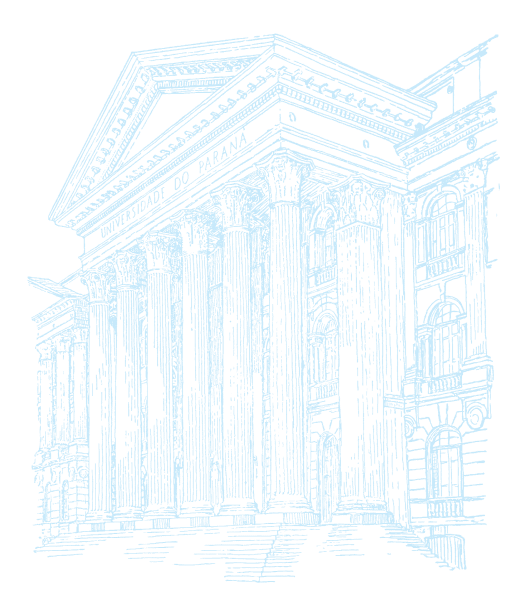
\includegraphics[width = \paperwidth]{Imagens/capa_UFPR}};
		\end{tikzpicture}
		\center
		%    \ABNTEXchapterfont 
		\MakeUppercase\imprimirinstituicao \vspace{-2mm}
		
		%\ifthenelse{\equal \ImprimirSetor{}}{}{
			%    \ABNTEXchapterfont 
		%	\MakeUppercase\ImprimirSetor}
		%\vspace{-2mm}
		
		%\ifthenelse{\equal \ImprimirProgramaPos{}}{}{
		%	     \ABNTEXchapterfont 
		%	\MakeUppercase\ImprimirProgramaPos}
		
		\ifthenelse{\equal \ImprimirCurso{}}{}{
			%    \ABNTEXchapterfont 
			\MakeUppercase\ImprimirCurso}
		
		\vspace{40mm}
		
		%    \ABNTEXchapterfont 
		\MakeUppercase\imprimirautor
		
		\vspace{40mm}
		%    \ABNTEXchapterfont
		\MakeUppercase\imprimirtitulo
		\vfill
		
		%\large
		\MakeUppercase\imprimirlocal
		
		%\large
		\imprimirdata
		
		\vspace*{10mm}
	\end{capa}
}

\pdfbookmark[0]{Capa}{Capa}
\imprimircapa


                             % Capa.

%---------------------------------------------------------------------
% FOLHA DE ROSTO
%---------------------------------------------------------------------

\makeatletter
\renewcommand{\folhaderostocontent}{
	\begin{center}
		
		%\vspace*{1cm}
		{
			%\ABNTEXchapterfont
			%\large
			\MakeUppercase\imprimirautor}
		
		\vspace*{\fill}%\vspace*{\fill}
		\begin{center}
			%      \ABNTEXchapterfont
			%\bfseries
			%\Large
			\MakeUppercase\imprimirtitulo
		\end{center}
		\vspace*{\fill}
		
		\abntex@ifnotempty{\imprimirpreambulo}{%
			\hspace{.45\textwidth}
			\begin{minipage}{.5\textwidth}
				\SingleSpacing\small
				\imprimirpreambulo.\vspace*{2mm}
				
				\abntex@ifnotempty{\imprimirorientador}
				{\imprimirorientadorRotulo~\imprimirorientador}
				\ifthenelse{\equal{\imprimirorientador}{}}
				{\imprimirorientadoraRotulo~\imprimirorientadora}
				{}
				\abntex@ifnotempty{\imprimircoorientador}
				{\par\imprimircoorientadorRotulo~\imprimircoorientador}%
				{\abntex@ifnotempty{\imprimircoorientadora}
					{\par\imprimircoorientadoraRotulo~\imprimircoorientadora}%
				}
				\ifthenelse{\equal{\imprimirscoorientadora}{} \AND \equal{\imprimirscoorientador}{}}{}
				{
					\ifthenelse{\equal{\imprimirscoorientador}{}}{}
					{\par\imprimirscoorientadorRotulo~\imprimirscoorientador}
					\ifthenelse{\equal{\imprimirscoorientadora}{}}{}
					{\par\imprimirscoorientadoraRotulo~\imprimirscoorientadora}
				}%
				%
			\end{minipage}%
			\vspace*{\fill}
		}%
		
		\vspace*{\fill}
		
		
		{  \MakeUppercase\imprimirlocal}
		\par
		{    \imprimirdata}
		\vspace*{1cm}
		
	\end{center}
}
\makeatother

\imprimirfolhaderosto*


                   % Folha de rosto.

%---------------------------------------------------------------------
% FICHA CATALOGRÁFICA
%---------------------------------------------------------------------

% São duas opções possíveis: usar um PDF pronto ou usar o comando abaixo. Se quiser usar o PDF, basta inserir um arquivo .pdf na pasta "Pré" chamado "Ficha catalográfica". Caso queira usar o comando, basta editá-lo abaixo de acordo com suas necessidades e depois remover o .pdf da pasta "Pré".

\newcommand{\PalavraschaveTexto}{Comércio internacional. Desigualdade de renda. Pobreza. Equilíbrio Geral Computável. Microssimulação.}

\newcommand{\insereFichaCatalografica}{ 
		\IfFileExists{Pré/Ficha catalográfica.pdf}
		{\includepdf[pages=-]{Pré/Ficha catalográfica.pdf}}
		{
			\begin{fichacatalografica}%\color{blue}
			\vspace*{\fill}					% Posição vertical
			\hrule							% Linha horizontal
			\begin{center}					% Minipage Centralizado
				\begin{minipage}[c]{12.5cm}		% Largura
					
					Luz, Felipe Duplat
					
					\hspace{0.5cm} \imprimirtitulo  / \imprimirautor. --
					\imprimirlocal, \imprimirdata.
					
					\hspace{0.5cm} \pageref{LastPage} p. : il. color \\
					
					\hspace{0.5cm} \imprimirtipotrabalho (mestrado) - \imprimirinstituicao. \ImprimirProgramaPos, do \ImprimirSetor. \\ 
					
					\hspace{0.5cm} Orientador: \imprimirorientador \\
					
					\hspace{0.5cm} Coorientadora: \imprimircoorientadora \\
					
					\hspace{0.5cm} Defesa: \imprimirlocal, \imprimirdata. \\
					
					\begin{minipage}{.96\textwidth}
						\hspace{0.5cm} 1. \PalavraschaveTexto. I. \imprimirinstituicao. \ImprimirSetor. \ImprimirProgramaPos. II. \imprimirorientador. III. \imprimircoorientadora. IV. \imprimirtitulo\\ 
						
						\hspace{92mm} CDU \imprimircdu \\
					\end{minipage}
				\end{minipage}
			\end{center}
			\hrule
		\end{fichacatalografica}
	}
}

\insereFichaCatalografica
\cleardoublepage


             % Ficha catalográfica.
%
%---------------------------------------------------------------------
% ERRATA
%---------------------------------------------------------------------

\chapter*{Errata}
\pdfbookmark[0]{Errata}{Errata}

Elemento opcional:
	\vspace{\onelineskip}
	
	FERRIGNO, C. R. A. \textbf{Tratamento de neoplasias ósseas apendiculares com
		reimplantação de enxerto ósseo autólogo autoclavado associado ao plasma
		rico em plaquetas}: estudo crítico na cirurgia de preservação de membro em
	cães. 2011. 128 f. Tese (Livre-Docência) - Faculdade de Medicina Veterinária e
	Zootecnia, Universidade de São Paulo, São Paulo, 2011.
	
	\begin{table}[htb]
		\center
		\footnotesize
		\begin{tabular}{|p{1.4cm}|p{1cm}|p{3cm}|p{3cm}|}
			\hline
			\textbf{Folha} & \textbf{Linha}  & \textbf{Onde se lê}  & \textbf{Leia-se}  \\
			\hline
			1 & 10 & auto-conclavo & autoconclavo\\
			\hline
		\end{tabular}
\end{table}


                          % Errata.
%
%---------------------------------------------------------------------
% TERMO DE APROVAÇÃO
%---------------------------------------------------------------------

% São duas opções possíveis: usar um PDF pronto ou usar o comando abaixo. Se quiser usar o PDF, basta substituir o arquivo .pdf na pasta "Pré". Caso queira usar o comando, basta editá-lo de acordo com suas necessidades e depois remover o .pdf da pasta "Pré".

\newcommand{\insereAprovacao}{
	\IfFileExists{Pré/Termo de aprovação.pdf}
	{\includepdf[pages=-]{Pré/Termo de aprovação.pdf}}
	{
		\begin{folhadeaprovacao}%\color{blue}
			
			\begin{center}
				{\ABNTEXchapterfont
					{\large\bfseries\MakeUppercase\folhadeaprovacaoname}\par\phantom{}\par
					%\large
					\MakeUppercase\imprimirautor}
				
				\vspace*{\fill}\vspace*{\fill}
				\begin{center}
					\ABNTEXchapterfont
					%\bfseries\Large
					\MakeUppercase\imprimirtitulo
				\end{center}
				\vspace*{\fill}
				\begin{minipage}{\textwidth}
					\hspace{.45\textwidth}
					\begin{minipage}{.5\textwidth}
						\imprimirpreambulo pela seguinte banca examinadora:
					\end{minipage}%
				\end{minipage}
				
				
				\vspace*{\fill}
			\end{center}
			\assinatura{{
					\ifthenelse{\equal{\imprimirorientador}{}}
					{\imprimirorientadora \\ Orientadora}
					{\imprimirorientador \\ Orientador}}
			}
			\assinatura{
				{Kênia Barreiro de Souza} \\ Co-orientadora}
			\assinatura{%\textbf
				{Professor(a)} \\ Universidade XXX}
			\assinatura{%\textbf
				{Professor(a)} \\ Universidade XXX}
			%\assinatura{%\textbf{Professor} \\ Convidado 4}
			
			\begin{center}
				\vspace*{0.5cm}
				%{\large\imprimirlocal}
				%\par
				%{\large\imprimirdata}
				\imprimirlocal, \imprimirDataDefesa.
				\vspace*{1cm}
			\end{center}
			
		\end{folhadeaprovacao}
	}
}

\insereAprovacao


              % Termo de aprovação.
%
%---------------------------------------------------------------------
% DEDICATÓRIA
%---------------------------------------------------------------------

\begin{dedicatoria}
	\vspace*{\fill}
	\centering
	\noindent
	
	\textit{Eu dedico...}
	
	\vspace*{\fill}
\end{dedicatoria}


                     % Dedicatória.

%---------------------------------------------------------------------
% AGRADECIMENTOS
%---------------------------------------------------------------------

\begin{agradecimentos}
	À minha irmã, Mariane, por todo o carinho e apoio durante esta jornada. À minha namorada, Maria Eduarda, pelo amor e incentivo que foram essenciais para eu chegar até aqui. Às amizades feitas dentro e fora do PPGDE pelo companheirismo e por terem tornado essa trajetória muito especial à sua própria maneira. Aos irmãos que Curitiba me deu, André Brito e Matheus Canhete, por toda solidariedade prestada desde o primeiro dia e pela feliz amizade. Ao Prof. Vinícius Vale por todos os ensinamentos, pela paciência e orientação ao longo destes últimos dois anos. À Profa. Kênia Souza pela coorientação que, sem dúvidas, elevou substancialmente a qualidade deste trabalho. Ao Núcleo de Estudos em Desenvolvimento Urbano e Regional (NEDUR) pela oportunidade de me engajar em projetos de pesquisa e de extensão que me ensinaram muito. À Coordenação de Aperfeiçoamento de Pessoal de Nível Superior (CAPES) pelo apoio financeiro concedido por meio da bolsa de mestrado. Aos servidores e funcionários da UFPR por todo o suporte durante essa trajetória acadêmica.
\end{agradecimentos}


                  % Agradecimentos.
%
%---------------------------------------------------------------------
% EPÍGRAFE
%---------------------------------------------------------------------

\begin{epigrafe}
	\vspace*{\fill}
	\begin{flushright}
		\textit{``as  elites são patrimonialistas e conservadoras, a classe média \\ é meritocrática e o povo? o povo não é nada!''}
	\end{flushright}
\end{epigrafe}


                        % Epígrafe.

%---------------------------------------------------------------------
% RESUMO
%---------------------------------------------------------------------

% PT-BR:
\begin{resumo}
	\SingleSpacing
	
	Apesar dos modelos teóricos de economia internacional convergirem para a compreensão de que o comércio pode ser um fator positivo para o desenvolvimento econômico de um país com \textit{spillovers} positivos sobre seus indicadores de desigualdade de renda e pobreza, as evidências empíricas apontam para distintos cenários, sem haver consenso na literatura econômica sobre seus efeitos. Isso não indica, necessariamente, que os resultados sejam inconclusivos, mas sim que não existe uma resposta única para a questão. Dado esse cenário, a presente dissertação tem como objetivo estimar os efeitos de uma maior abertura comercial sobre a distribuição da renda familiar e sobre os índices de pobreza no Brasil. Para isso, utiliza-se um modelo nacional de equilíbrio geral para simular os efeitos de curto-prazo de uma redução tarifária em 10\% integrado a uma abordagem de microssimulações contrafactuais para capturar as respostas comportamentais dos indivíduos. Os resultados indicaram que o comércio internacional exerce pouca influência sobre os indicadores de desigualdade de renda e pobreza. As variações registradas foram bastante modestas, sobretudo tratando-se do efeito sobre a pobreza extrema e sobre a desigualdade de renda, sendo praticamente nulo. Uma possível razão que explique esse resultado esteja no fato que as barreiras tarifárias brasileiras já não são altas o suficiente para que uma nova redução tarifária consiga impor efeitos expressivos sobre os indicadores observados.
	
	\noindent 
	\textbf{Palavras-chaves}: Comércio internacional. Desigualdade de renda. Pobreza. Equilíbrio Geral Computável. Microssimulação comportamental.
\end{resumo}


                           % Resumo.

%---------------------------------------------------------------------
% ABSTRACT
%---------------------------------------------------------------------

% ENG:
\begin{resumo}[Abstract]
	\begin{otherlanguage*}{english}
		\SingleSpacing
		
		Despite theoretical models of international economics converging on the understanding that trade can be a positive factor for the economic development of a country, with positive spillovers on its indicators of income inequality and poverty, empirical evidence points to distinct scenarios, without a consensus in the economic literature about their effects. This does not necessarily indicate that the results are inconclusive, but rather that there is no single answer to the question. Given this scenario, the present dissertation aims to estimate the effects of greater trade openness on the distribution of family income and on poverty rates in Brazil through a national general equilibrium model, simulating the short-term effects of a tariff reduction by 10\%, integrated with a counterfactual microsimulations approach to capture individuals' behavioral responses. The results indicated that international trade has little influence on indicators of income inequality and poverty. The recorded variations were quite modest, especially when it comes to the effect on extreme poverty and income inequality, which was practically negligible. A possible reason that explains this result is the fact that Brazilian tariff barriers are no longer high enough for a new tariff reduction to impose significant effects on the observed indicators.
		
		\noindent 
		\textbf{Keywords}: International trade. Wage inequality. Poverty. Computable General Equilibrium. Behavioral microsimulation.
	\end{otherlanguage*}
\end{resumo}


                         % Abstract.

%---------------------------------------------------------------------
% LISTAS
%---------------------------------------------------------------------

% Lista de figuras:
\pdfbookmark[0]{\listfigurename}{lof}
\listoffigures*
\cleardoublepage



% Lista de quadros:
\pdfbookmark[0]{Lista de quadros}{loq}
\listofquadros*
\cleardoublepage



% Lista de tabelas:
\pdfbookmark[0]{\listtablename}{lot}
\listoftables*
\cleardoublepage



% Lista de abreviaturas e símbolos:
\begin{siglas}
	
	\item[H-O]      Modelo Heckscher-Ohlin.
	
	\item[SS]       Teorema Stolper-Samuelson.
	
	\item[EGC]      Equilíbrio Geral Computável.
	
	\item[PNAD]     Pesquisa Nacional por Amostragem de Domicílio.
	
	\item[PNADc]    Pesquisa Nacional por Amostragem de Domicílio Contínua.
	
	\item[POF]      Pesquisa de Orçamentos Familiares.
	
	\item[ALCA]     Área de Livre-Comércio das Américas.
	
	\item[OMC]      Organização Mundial do Comércio.
	
	\item[SCN]      Sistema de Contas Nacionais.
	
	\item[Mercosul] Mercado Comum do Sul.
	
	\item[UE]       União Europeia.
	
	\item[CES]      \textit{Constant Elasticity of Substitution} -- Elasticidade de Substituição Constante.
	
	\item[LES]      \textit{Linear Expenditure System} -- Sistema de Despesa Linear.
	
	\item[FGT]      \textit{Foster-Greer-Thorbecke}.
\end{siglas}


% Símbolos:
%\begin{simbolos}
%	\item[$\alpha$] Letra grega Alfa em minúsculo.
%	\item[$\beta$]  Letra grega Beta em minúsculo.
%	\item[$\gamma$] Letra grega gama em minúsculo.
%\end{simbolos}



% Sumário:

% tamanho de fonte para sumário:
\newcommand{\tocfont}{\normalsize}

% Modifica o espaçamento:
\setlength{\cftbeforechapterskip}{18pt}
\setlength{\cftbeforesectionskip}{5pt}
\setlength{\cftbeforesubsectionskip}{0pt}
\setlength{\cftbeforesubsubsectionskip}{0pt}
\setlength{\cftbeforeparagraphskip}{0pt}

%% Altera a indentação:
%\cftsetindents{chapter}{0pt}{42pt}
%\cftsetindents{section}{0pt}{42pt}
%\cftsetindents{subsection}{0pt}{42pt}
%\cftsetindents{subsubsection}{0pt}{42pt}

% Gerar sumário:
\pdfbookmark[0]{\contentsname}{toc}
\tableofcontents*


                           % Listas de figuras, quadros, tabelas e sumário.



% ----------------------------------------------------------
% ELEMENTOS TEXTUAIS
% ----------------------------------------------------------
\textual


% ----------------------------------------------------------
% CAPÍTULO 01 - INTRODUÇÃO
% ----------------------------------------------------------

% limpar customização do cabeçalho:
\pagestyle{fancy}
\fancyhf{}
\fancyhead[R]{\small\thepage}
\renewcommand{\headrulewidth}{0pt}

\chapter{Introdução} \label{cha:introducao}

Há uma extensa literatura que busca analisar o canal de transmissão entre comércio internacional e a desigualdade de renda e pobreza \cite{ferreira06, castilho12, bayar17, anderson20}. Esse debate é motivado, por um lado, pelo crescente destaque da abertura comercial como um vetor para o crescimento econômico \cite{atkin22} e, por outro lado, pela crença que essa abertura é capaz de gerar melhorias sobre a produtividade e renda, com repercussões positivas nos indicadores de desigualdade de renda e pobreza\footnote{Vale ressaltar, embora seja reconhecido o caráter multidimensional da pobreza, dentro do escopo do trabalho proposto, a pobreza será tratada exclusivamente como equivalente à insuficiência de renda.} \cite{carneiro06}.

A maioria dos modelos teóricos de economia internacional apontam, por sua vez, que o comércio é capaz de influir nos preços relativos de um país, gerando fortes efeitos distributivos. Com isso, espera-se que haja grupos beneficiados e grupos prejudicados a partir de uma determinada abertura comercial. Entretanto, esses modelos também apontam que os ganhos serão grandes o suficiente para compensar as perdas ocasionadas, dado o aumento de produtividade e bem-estar gerados pela maior exposição ao comércio internacional. O modelo H-O \cite{heckscher49, ohlin67} e o Teorema SS \cite{stolper41}, derivado do modelo anterior, são dois exemplos que ilustram essa dinâmica.

No modelo H-O, a abertura comercial promove mudanças nos preços relativos. Os bens que são intensivos no uso do fator produtivo abundante no país terão seus preços relativos aumentados, pois a demanda por esses bens aumenta no mercado internacional; ao passo que os preços relativos dos bens que são intensivos no uso do fator de produção escasso tendem a diminuir. O resultado é a especialização do país no bem que usa intensivamente seu fator produtivo abundante, tornando por exportá-lo. O bem que usa mais intensivamente seu fator escasso é importado \cite{heckscher49, ohlin67}. Essa mudança de preços relativos, de acordo com o modelo, promove o aumento da eficiência tanto na produção quanto no consumo dos países, elevando seu nível de bem-estar.

Entretanto, esse ganho de bem-estar não é igualmente repartido na sociedade. De acordo com o teorema SS, o aumento do preço relativo de um bem, via efeito magnificação\footnote{Qualquer mudança nos preços dos produtos gera um efeito ainda maior no preço dos fatores produtivos \cite{jones65}}, também eleva a remuneração relativa do seu fator produtivo, reduzindo, por conseguinte, a remuneração do outro fator \cite{stolper41}. Ou seja, o aumento da renda dos proprietários de um fator produtivo resulta diretamente na redução da renda dos proprietários do outro fator. Essa conclusão nos permite afirmar que o comércio internacional gera vencedores e perdedores.

Contudo, isso não significa que as perdas não possam ser compensadas. Se os ganhos excedem as perdas no movimento de liberalização comercial, é possível redistribuir os ganhos de tal forma que todos os indivíduos tenham, pelo menos, tanto quanto já tinham antes da referida liberalização. A isso, a teoria econômica conceitua como \textit{princípio da compensação} \cite{irwin98}, sendo entendida enquanto a escolha política e econômica sobre como lidar com os custos de uma liberalização comercial. Esta pode assumir diversas formas, incluindo pagamentos diretos, seguro salarial, retreinamento profissional ou até ajuda na transição para um novo emprego \cite{kolben21}. Ou seja, é a política preferencial a ser seguida para maximizar o bem-estar dada uma determinada uma abertura comercial.

Desse modo, pode-se afirmar que a teoria econômica converge para a compreensão de que o comércio internacional, mesmo ocasionando perdedores, é capaz de gerar efeitos suficientemente positivos para que, uma vez redistribuídos, coloquem todos os indivíduos numa situação pelo menos tão boa quanta era na situação de autarquia, com repercussões positivas sobre os indicadores de desigualdade de renda e pobreza.

Entretanto, as evidências empíricas apontam para distintos cenários sem encontrar a mesma convergência \cite{winters04}. Para os países latino-americanos, em especial o Brasil, essa questão é ainda mais dúbia, já que uma economia em desenvolvimento mais integrada ao comércio internacional também pode estar mais vulnerável a choques externos, como mudanças abruptas nos termos de troca, que podem reduzir significativamente o crescimento do país \cite{bannisterthugge01}. Essa vulnerabilidade eleva o grau de incerteza, fazendo com que o país possa operar com níveis de pobreza acima do que uma economia menos integrada operaria, além de gerar uma perda da eficiência de políticas econômicas capazes de reduzir pobreza e desigualdade de renda \cite{winters02}.

Uma das possíveis explicações para essas divergências está relacionada a estrutura produtiva de cada país, assim como a relação entre a estrutura produtiva e a distribuição de renda. A forma que essa diversidade de fatores pode gerar distintos impactos em termos de desigualdade de renda e pobreza é uma questão pouco explorada na literatura e, possivelmente, a razão da referida ausência de consenso. A grande maioria dos estudos se limitou a abordar o tema a partir das experiências históricas de abertura comercial - sendo comumente utilizados modelos de equilíbrio parcial \cite{castilho12, bayar17} - ou a partir de estudos de caso, sem focar na questão estrutural \cite{borrazetal12, estrades12, campostimini22}. Desse modo, pouco se debateu na literatura sobre a influência do padrão de comércio e o perfil da pauta exportadora, bem como do padrão de consumo e renda das famílias, sobre a desigualdade de renda e pobreza, evidenciando os canais de transmissão que podem influenciar esses indicadores. 

Por essa razão, a presente dissertação tem como objetivo estimar os efeitos de uma maior abertura comercial sobre a distribuição da renda familiar e sobre os índices de desigualdade de renda e pobreza no Brasil. Para isso, utiliza-se um modelo nacional de equilíbrio geral integrado a uma abordagem de microssimulação contrafactual\footnote{Optou-se por utilizar esses dois modelos porque seu uso conjunto torna por corrigir as limitações de ambos. Essa discussão é aprofundada no Capítulo~\ref{cha:metodologia}.} referentes ao ano de 2015. O primeiro cumpre o papel de calcular os efeitos macroeconômicos e setoriais de uma redução tarifária na magnitude de 10\%, enquanto que, por meio do segundo, é possível estimar esses efeitos a nível individual, calculando o impacto sobre a desigualdade de renda e pobreza.

Existe uma grande vantagem em trabalhar com modelos de equilíbrio geral para estudos sobre desigualdade de renda e pobreza em comparação a modelos de equilíbrio parcial. Sua estrutura é capaz de captar mais eficientemente os efeitos de reformas comerciais, especialmente sobre salários e emprego -- determinantes do impacto geral de aberturas comerciais \cite{naranpanawa11}. Além disso, não há problemas comuns de abordagens econométricas como, por exemplo, viés de seleção, heterogenidade e dificuldade em separar os efeitos de múltiplas reformas introduzidas simultaneamente \cite{anderson20}.

O Brasil serve como um interessante estudo de caso por duas razões. Primeiro, pelo recente histórico de abertura comercial, seguindo a tendência de diversos países em desenvolvimento que, nas últimas quatro décadas, implementaram uma série de políticas liberalizantes em larga escala, integrando-se ao sistema de comércio global \cite{pavcnik17}, embora seu coeficiente de abertura comercial seja um dos menores do mundo\footnote{\textcite{ourworldindata}.}. Segundo, o Brasil ainda é um país com elevados índices de desigualdade de renda e pobreza, apesar da queda acentuada desde o início da década de 2000 \cite{ocde15}.

Até onde se tem conhecimento, apenas \textcite{carneiro06, ferreira06} conduziram um estudo semelhante para o Brasil, entretanto, sem realizar o mesmo nível de desagregação das famílias por percentis de renda. Esta dissertação contribui para a literatura econômica ao incorporar os efeitos do comércio internacional sobre a estrutura de renda das diferentes classes de famílias brasileiras, com os dados mais recentes e elevado detalhamento de informações sobre a distribuição funcional da renda e consumo das famílias.

Esta dissertação segue a seguinte ordem: após a Introdução, o segundo capítulo aborda a literatura acerca da interação entre o comércio internacional e os indicadores de desigualdade de renda e pobreza. O terceiro capítulo detalha a estratégia empírica adotada. O quarto capítulo detalha os resultados obtidos. O último capítulo apresenta as considerações finais.




% ----------------------------------------------------------
% CAPÍTULO 02 - REVISÃO DE LITERATURA
% ----------------------------------------------------------

\chapter{Revisão de literatura}\label{cha:revisao_de_literatura}

Este capítulo contextualiza as contribuições, tanto teóricas quanto empíricas, da literatura econômica sobre os efeitos do comércio internacional sobre a desigualdade de renda e pobreza. A primeira seção discute as contribuições teóricas, concentrando-se nos canais de transmissão que associam o comércio internacional à desigualdade e pobreza. Nele, discute-se a natureza desse vínculo e os comportamentos esperados. A segunda e última seção apresenta as evidências empíricas existentes sobre os referidos canais de transmissão e os distintos cenários apontados.



\section{Os canais de transmissão}\label{sec:canais_de_transmissao}

De início, é importante afirmar que estabelecer uma associação entre comércio internacional e indicadores de desigualdade de renda e pobreza é uma atividade desafiadora. A própria mensuração de desigualdade e pobreza é bastante complexa, sendo, por si só, tema exclusivo de diversos estudos \cite{neri06, soares09, hoffmann19}. Ademais, há outro grande desafio em desvincilhar os próprios canais de transmissão entre si, uma vez que são interdependentes e sujeitos a influência de outros tipos de políticas e eventos econômicos \cite{bannisterthugge01}.

Pode-se entender o comércio internacional enquanto um choque exógeno sobre os preços relativos de uma economia que, segundo \textcite{winters02}, gera fortes efeitos distributivos entre e dentro dos países. O comércio internacional pode afetar os preços relativos de uma economia de diversas formas: por variações cambiais, inovação, concorrência, etc. No modelo H-O, a abertura comercial promove a convergência dos preços relativos entre os dois países a partir da entrada do bem por um preço abaixo do praticado em autarquia.

Para o autor, o resultado final desse choque depende da estrutura de mercado e particularmente do setor de distribuição -- entendido enquanto uma categoria genérica para agrupar todos os canais de transmissão existentes em uma economia \cite{winters02}. Entretanto, frente a um processo de liberalização comercial, se a estrutura de mercado e setor de distribuição performam aquém do esperado, é possível que haja determinadas regiões do país e setores produtivos que fiquem isolados dos efeitos positivos desse processo \cite{bannisterthugge01}.

Intuitivamente, o primeiro canal de transmissão entre o comércio internacional e a desigualdade de renda e pobreza que se pode imaginar é o crescimento econômico, uma vez que um maior crescimento indica maiores oportunidades de emprego e de geração de renda, que afetam diretamente a pobreza e desigualdade\footnote{Há uma extensa literatura econômica acerca dos efeitos do crescimento pró-pobre e pró-rico (\textit{pro-poor and pro-rich growth}) sobre a desigualdade de renda. A respeito disso, pode-se citar \textcite{ravallion04, thorbecke22}.}. Entretanto, sua conexão com o comércio internacional é indefinida, sendo também, por si só, tema de diversos estudos \cite{anderson16, dix17, gnangnon18}. Em razão disso, ignora-se aqui o crescimento econômico como possível canal de transmissão. 

A primeira subseção discute os canais de transmissão conhecidos na literatura entre o comércio internacional e a desigualdade de renda. Já a segunda subseção discute os canais de transmissão que afetam a pobreza. O Quadro~\ref{quad:canais_de_transmissao} resume em tópicos a discussão realizada a seguir.

\begin{quadro}[h]
	\begin{threeparttable}
		\centering
		\caption{Canais de transmissão entre comércio internacional e a desigualdade de renda e pobreza}
		\footnotesize
		\label{quad:canais_de_transmissao}
		\begin{tabular}{|| m{7.5cm} | m{7.5cm} ||}
			\hline \hline
			\multicolumn{1}{||c|}{\textbf{desigualdade de renda}} & \multicolumn{1}{c||}{\textbf{pobreza}} \\ \hline
			\begin{itemize}
				\item prêmio salarial por qualificação
				\item prêmio salarial por setor
				\item emprego informal
				\item imperfeições do mercado de crédito
				\item quantidade de bens não-negociáveis
			\end{itemize} &
			\vspace{0.2cm}
			alteração no:
			\begin{itemize}
			\item preço e acesso dos produtos negociáveis
			\item preço relativo dos fatores de produção
			\item receitas e capacidade de gastos do governo
			\item incentivos de investimentos e inovação
			\item vulnerabilidade a choques externos
			\end{itemize} \\ \hline \hline
		\end{tabular}
		\begin{tablenotes}
			\scriptsize
			\item Fonte: \textcite{bannisterthugge01, xu03, goldbergpavcnik04, banerjee04}.
		\end{tablenotes}
	\end{threeparttable}
\end{quadro}


\subsection{Desigualdade de renda} \label{subsec:desigualdade_de_renda}

Analisando a desigualdade de renda, o primeiro ponto do Quadro~\ref{quad:canais_de_transmissao} se refere ao prêmio salarial por qualificação. Este pode ser entendido a diferenciação nos salários devido ao nível de qualificação, habilidades ou educação de um trabalhador. Políticas comerciais podem afetar o prêmio salarial a partir de: 1- um aumento nos retornos de determinadas ocupações associadas a um nível de escolaridade maior; 2- um deslocamento da produção de bens intermediários intensivos em qualificação dos países desenvolvidos para os em desenvolvimento; 3- uma mudança tecnológica com viés para maior qualificação; e 4- uma alteração da composição nos produtos produzidos dentro das indústrias em prol dos intensivos em trabalho qualificado \cite{goldbergpavcnik04}.

De acordo com \textcite{goldbergpavcnik04}, seu comportamento é positivamente relacionado com os indicadores de desigualdade. Ou seja, uma redução no prêmio salarial por qualificação diminui a desigualdade de renda. Isso ocorre porque o prêmio salarial afeta diretamente o \textit{gap} entre dois ou vários salários, agravando a desigualdade de renda. Esse comportamento é convergente com os modelos teóricos de comércio internacional, em especial com o modelo H-O - considerando dois países, desenvolvido e em desenvolvimento, cujo primeiro país é abundante em trabalho qualificado e o segundo, em não-qualificado, o teorema SS garante que haveria uma redução salarial dos trabalhadores qualificados, aumentando o dos não-qualificados quando ambos se engajam em comércio.

Em segundo, o Quadro~\ref{quad:canais_de_transmissao} cita o prêmio salarial por setor como outro possível canal de transmissão. Segundo \textcite{goldbergpavcnik04}, este se refere enquanto a variação salarial que pode existir entre trabalhadores empregados em setores diferentes da atividade econômica. Há duas formas que políticas comerciais podem afetar o prêmio por setor. Primeiro, rigidez na mobilidade do fator trabalho. Modelos de comércio de curto-prazo com a referida rigidez apontam que reduções tarifárias tornam por diminuir o prêmio salarial por setor \cite{heckman00}. Isso pode ocorrer em mercados de concorrência perfeita ou imperfeita \cite{harrison03}. Segundo, mudanças de produtividade intersetorial. Supondo que o comércio internacional possa aumentar a produtividade de um país, esta pode ser revertida em aumento no prêmio por setor desde que possa aumentar o salário dos trabalhadores \cite{hay01}.

Conforme \textcite{goldbergpavcnik04}, seu comportamento é negativamente relacionado com a desigualdade de renda. Ou seja, uma redução do prêmio por setor torna por elevar o \textit{gap} salarial. Isso pode acontecer se uma abertura comercial tornar por reduzir o prêmio. Isto pode aumentar a desigualdade caso os setores mais afetados pela abertura sejam intensivos em trabalho não qualificado \cite{pavcnik04}.

Em terceiro, o Quadro~\ref{quad:canais_de_transmissao} elenca o emprego informal. A informalidade também é um canal de transmissão capaz de influir sobre os indicadores de desigualdade de renda. Isso acontece porque, segundo \textcite{goldbergpavcnik04}, uma abertura comercial pode ser capaz de expandir o tamanho do mercado informal de um país \cite{goldberg03}. Uma vez que os trabalhadores informais estão associados a menores salários e qualidade da infraestrutura do trabalho \cite{bargain14}, é possível afirmar que seu comportamento é positivamente relacionado com os indicadores de desigualdade de renda. Ou seja, uma abertura comercial pode aumentar a informalidade, causando o aumento da desigualdade de renda.

Em quarto, cita-se o mercado de crédito. Ele pode ser influenciado pelo comércio internacional, sendo, também, um canal de transmissão sobre a desigualdade. De acordo com \textcite{goldbergpavcnik04}, sua eficiência é negativamente relacionada com os indicadores de desigualdade de renda.

\textcite{banerjee04} desenvolvem um modelo dinâmico de comércio internacional com fatores específicos que incorpora imperfeição na mobilidade do capital e trabalho -- só há a transição de trabalho para capital se o indivíduo tiver uma quantidade mínima de capital humano. Frente a uma abertura comercial, observa-se o aumento da taxa de juros nos países com mercado de crédito mais robusto e consequente aumento da produtividade média, ao passo que os países com mercado de crédito pouco eficiente sofrem uma redução em sua taxa de juros, fazendo com que o capital permaneça nos setores menos produtivos - uma vez que aumenta a probabilidade de inadimplência. O efeito sobre a distribuição de renda é um \textit{trade-off} para os países em desenvolvimento: maior crescimento econômico no longo prazo às custas de alta volatilidade no curto-prazo.

O último canal de transmissão listado é o que a literatura econômica chama de bens não-negociáveis. Entende-se por isso todos os bens cuja características dificultam ou impedem de serem exportados ou importados. \textcite{xu03}, utilizando um um modelo H-O com dois países (norte e sul), dois fatores (trabalho qualificado e não-qualificado) e quatro bens (1, 2, 3 e 4 numa escala crescente de complexidade), argumenta que os efeitos da abertura comercial sobre a desigualdade de renda nos países em desenvolvimento são em forma de U. Para níveis de proteção comercial inicialmente elevados, a abertura reduz a desigualdade, enquanto para níveis de proteção mais baixos, a abertura aumenta a desigualdade.

Isso ocorre por causa da gama de bens não-negociáveis: a proteção comercial transforma alguns bens negociáveis em não-negociáveis via distorção nas vantagens comparativas. Se esses bens são intensivos em trabalho qualificado, uma progressiva abertura comercial, via redução tarifária, aumenta os incentivos para importar. A consequência disso é a redução do salário do trabalho qualificado no país, reduzindo o \textit{gap} salarial - como visto no Teorema SS. Entretanto, a redução tarifária também provoca a piora dos termos de troca, o que torna por incentivar as exportações do país - o que elevaria o salário do trabalho qualificado, aumentando a desigualdade. Uma elevada abertura comercial faria com que o "efeito exportação" superasse o "efeito importação", criando, por conseguinte, a forma de U para os países em desenvolvimento \cite{goldbergpavcnik04}.


\subsection{Pobreza} \label{subsec:pobreza}

A segunda coluna do Quadro~\ref{quad:canais_de_transmissao} lista os canais de transmissão entre o comércio internacional e os indicadores de pobreza. Os indivíduos mais pobres podem ser beneficiados por uma abertura comercial, a partir da redução do preço dos bens importados, como alimentos básicos e farmacêuticos, gerando o aumento da renda real, além de aumentar o acesso a novos bens de consumo \cite{bannisterthugge01}. Como geralmente os indivíduos mais pobres são produtores líquidos de bens voltados para a exportação (como na Agricultura, por exemplo), o aumento da demanda por exportações pode elevar o preço dos produtos e, por conseguinte, estimular o aumento da produção, emprego e renda do setor \cite{bannisterthugge01}.

A alteração no preço relativo dos fatores de produção, como apresenta o Quadro~\ref{quad:canais_de_transmissao}, também é um canal de transmissão sobre os indicadores de pobreza, uma vez que afeta diretamente a remuneração do trabalho qualificado e não-qualificado. Como já visto no modelo H-O, o comércio internacional pode beneficiar os mais pobres caso a abertura se reverta numa elevação da produtividade marginal do trabalho não-qualificado \cite{bannisterthugge01}.

O Quadro~\ref{quad:canais_de_transmissao} cita as receitas e capacidade de gastos do governo como outro canal de transmissão para o comércio internacional. Isso ocorre porque políticas de liberalização comercial, feitas por meio de cortes tarifários, afetam diretamente as receitas tarifárias, o que pode prejudicar a capacidade de gastos do governo.

De acordo com \textcite{bannisterthugge01}, o efeito sobre a pobreza se baseia no argumento que essa redução na receita tarifária teria que ser compensada pelo governo por meio de cortes em programas sociais ou criação de novos impostos, afetando desproporcionalmente os mais pobres. Entretanto, o resultado é ambíguo, sendo dependente do valor inicial das tarifas. Caso sejam altas, o corte tarifário eleva o fluxo comercial de tal maneira a compensar as perdas tributárias, além de diminuir os incentivos ao contrabando e corrupção. Caso sejam suficientemente baixas, não é possível compensar a perda da receita tarifária.

Investimentos e inovação, citado no Quadro~\ref{quad:canais_de_transmissao}, também são um possível canal de transmissão. A literatura econômica associa reformas comerciais a maiores fluxos de investimento externo com \textit{spillovers} sobre tecnologias, novas práticas de negócios e outros efeitos sobre as empresas nacionais que aumentam o nível geral de produtividade\footnote{Reformas comerciais também resultam na melhoria da formação de capital humano, que gera um significante efeito sobre inovação \cite{bannisterthugge01}.} \cite{bannisterthugge01}. Entretanto, é possível que esse tipo de aumento de produtividade engendre um crescimento econômico que beneficie desproporcionalmente os mais ricos, o que agravaria os indicadores de pobreza \cite{lundberg03}.

O último canal de transmissão listado no Quadro~\ref{quad:canais_de_transmissao} se refere a vulnerabilidade a choques externos. Aberturas comerciais podem facilitar a diversificação da pauta exportadora de um país, tornando-o menos dependente de um único mercado ou bem; como pode, também, tornar a economia mais vulnerável a choques externos. O canal de transmissão com indicadores de pobreza, nesse caso, se dá quando esse choque recai sobre setores intensivos em trabalho não-qualificado, como Agricultura ou qualquer setor muito caracterizado por trabalho informal, afetando desproporcionalmente os mais pobres \cite{bannisterthugge01}. Desse modo, a abertura comercial gera efeitos ambíguos: há evidências de elevação do crescimento econômico, entretanto, com altos níveis de volatilidade macroeconômica - o que, mais uma vez, afeta desproporcionalmente os mais pobres.



\section{As evidências empíricas} \label{sec:evidencias_empiricas}

Conforme discutido no Capítulo~\ref{cha:introducao}, apesar da teoria econômica convergir para a noção que o comércio internacional é um fator capaz de reduzir a desigualdade de renda e pobreza, as evidências empíricas apontam para distintos cenários. \textcite{winters02} elenca cinco razões para o \textit{mismatch} entre a teoria e as evidências empíricas: 1- distribuição funcional da renda; 2- dimensionalidade dos modelos; 3- pressuposto de mobilidade dos fatores; 4- equilíbrio diverso; e 5- comportamento do preço dos bens não negociáveis para \textit{market-clearing}.

Para analisar esses distintos cenários, optou-se por apresentar a contribuição empírica a partir do aspecto metodológico. A primeira subseção discute as contribuições a partir de modelos de equilíbrio parcial e a segunda, a partir de modelos de equilíbrio geral. Essa divisão é adotada para proporcionar uma compreensão mais aprofundada de como essa escolha pode afetar, de algum modo, os resultados sobre desigualdade de renda e pobreza, como discutido em \textcite{anderson20}.


\subsection{Equilíbrio parcial} \label{subsec:eq_parcial}

Um dos mais tradicionais canais de transmissão, no equilíbrio parcial, é o mercado de trabalho. Nesse caminho, \textcite{borjas94} buscam verificar se a tendência de exposição dos setores altamente concentrados ao comércio internacional durante 1963 a 1988 nos Estados Unidos podem ser responsáveis por grande parte das tendências na desigualdade salarial. Usando um modelo de séries temporais, controlando pela experiência e escolaridade dos indivíduos, os autores encontraram evidências que a exposição ao mercado internacional elevou os indicadores de desigualdade de renda.

Já \textcite{forbes01} estima o efeito da elevação do fluxo comercial sobre a remuneração do trabalho qualificado e não-qualificado e sobre a desigualdade salarial utilizando os dados de 36 países de 1980 até 1995. A partir de um modelo de efeitos fixos, no qual mede a desigualdade salarial pela razão entre a remuneração dos trabalhadores qualificados e não-qualificados, as evidências sugerem que o comércio internacional aprofundou o \textit{gap} salarial, reduzindo o salário dos trabalhadores sem qualificação.

Seguindo a mesma linha, \textcite{galianisanguinetti03} analisam se a liberalização comercial teve algum impacto identificável na distribuição de salários no setor manufatureiro na Argentina durante os anos noventa. Especificamente, os autores testam se os setores que experimentaram um aumento da penetração das importações foram também aqueles no qual se observou uma elevação da desigualdade salarial. Utilizando um modelo de efeitos fixos, controlando pelas características dos indivíduos e do setor, a partir dos microdados nacionais, os resultados apontam que há evidências que a liberalização contribuiu para aprofundar a desigualdade de renda via aumento do prêmio salarial por qualificação. Entretanto, a liberalização explica apenas uma proporção relativamente pequena do aumento observado.

O aumento da desigualdade observado na Argentina também foi tema para \textcite{galianiporto11} que apresentam um modelo teórico com salários rígidos abaixo do nível competitivo - por conta da presença de sindicatos e abundância dos fatores produtivos. Utilizando microdados nacionais e um modelo de efeitos fixos para estimar o log salarial dos indivíduos, as evidências apontam que a abertura comercial reduz os salários e tarifas industriais reduzem o prêmio por qualificação na indústria, havendo, por conseguinte, uma redução da desigualdade comprimindo a média salarial. Entretanto, o resultado apenas converge por considerar a distorção dos preços causada pela presença dos sindicatos.

\textcite{castilho12} estudam o efeito da globalização\footnote{Definido pelas autoras como "um termo abrangente [...] para incluir a liberalização do comércio e a integração nos mercados mundiais" \cite{castilho12}.} sobre a desigualdade de renda e pobreza a nível estadual. Utilizando um modelo de efeitos fixos e os dados da PNAD para os anos de 1987 a 2005, as autoras calculam a exposição ao comércio internacional a partir dos indicadores de fluxo comercial (penetração das importações defasada e exposição às exportações defasada) e seu efeito sobre os índices de Gini, Theil e FGT. As evidências apontam que a abertura comercial brasileira contribuiu com a elevação da pobreza e desigualdade de renda nas áreas
urbanas, havendo também uma possibilidade de relação com uma redução observada na desigualdade e pobreza nas áreas rurais.

\textcite{bayar17} se propuseram a mensurar o grau e direção da interação entre globalização, pobreza e desigualdade de renda para onze países da América Latina por meio de testes de raiz unitária em painel -- sendo sua contribuição a nível metodológico. Usando índice de Gini, FGT e corrente de comércio como porcentagem do PIB para representar, respectivamente, as medidas de desigualade de renda, pobreza e abertura comercial, os autores afirmam que o comércio internacional, no longo-prazo, reduziu os indicadores de pobreza às custas do aumento da desigualdade de renda.

Considerando experiências históricas de abertura comercial, \textcite{borrazetal12} estudam os impactos da liberalização do comércio sobre desigualdade e pobreza, focando nos preços e salários como os canais de transmissão do comércio internacional. Utilizando o modelo baseado de \textcite{dixit80} estendido por \textcite{porto06}, os autores encontraram que o Uruguai se beneficiou com a redução do nível de pobreza, apesar de haver praticamente nenhum efeito sobre a desigualdade de renda. Já o Paraguai sofreu com o aumento dos indicadores de pobreza, mesmo tendo havido uma melhoria na desigualdade de renda.

Já \textcite{porto03} examina o impacto das reformas comerciais, tanto nacionais quanto estrangeiras ocorridas na Argentina sobre o nível de pobreza. A reforma nacional seria um corte tarifário no preço dos bens de capital e de consumo importados no valor de 2\% e 8\%; já a reforma estrangeira, aumento em 7,5\% e 15,4\% nos bens agro-manufaturados e 1,6\% e 7\% nos bens manufaturados industriais.

Utilizando uma especificação que incorpora a heterogeneidade familiar em um modelo de equilíbrio parcial, o fator trabalho é desagregado em qualificado e não-qualificado com as famílias consumindo bens negociáveis e não-negociáveis. Tal qual em \textcite{borrazetal12}, há dois canais de transmissão: preços e salários. A evidência aponta que a combinação das reformas poderia causar uma redução do índice FGT entre 1,6 a 4,6 p.p., sendo majoritariamente influenciada pelos efeitos marginais da reforma doméstica.

\subsection{Equilíbrio geral} \label{subsec:eq_geral}

Considerando as experiências históricas de abertura comercial, \textcite{carneiro06} avaliam o impacto de uma expansão da abertura comercial brasileira experimentada nos anos de 1990 sobre o emprego, pobreza e desigualdade utilizando um modelo estático de equilíbrio geral computável baseado em \textcite{robinson99}, com 42 setores referente ao ano de 1996, para simular diferentes cenários de políticas\footnote{São oito simulações, a saber: 1- $\uparrow$ 10\% produtividade; 2- $\uparrow$ 10\% preço das importações; 3 e 4- efeitos de uma mudança de 50\% nas tarifas de importação; 5- $\uparrow$ 10\% da taxa de subsídios às exportações; 6- avaliar os impactos da ALCA; 7- avaliar os impactos da OMC; e 8- $\downarrow$ 10\% câmbio.}. Seus resultados são levados para um modelo de microssimulação, baseado em \textcite{ganuza07}, a fim de avaliar os impactos de uma maior sobre a distribuição de renda e pobreza. A principal conclusão do artigo é que a liberalização comercial por si só não seria suficiente para reduzir a pobreza e a desigualdade no Brasil de forma significativa.

Analisando exercícios de simulação hipotética, \textcite{ferreira06} analisam os efeitos potencias da formação da ALCA sobre os níveis de pobreza e distribuição de renda brasileiros. É utilizado um modelo inter-regional estático de equilíbrio geral computável para o Brasil, calibrado a partir do SCN de 1996 com 42 setores e 52 bens. Os trabalhadores foram desagregados em dez níveis de acordo com a renda. A partir de uma integração com o modelo de microssimulação comportamental, as evidências indicaram que reduções tarifárias, por maiores que sejam, são incapazes de afetar a pobreza no Brasil.

\textcite{estrades12}, ao estimar os potenciais efeitos do acordo entre o Mercosul e a UE sobre a pobreza no Uruguai, analisa se a agenda externa do bloco é pró-pobre. Utilizou-se um modelo global de equilíbrio geral, MIRAGE, calibrado para o ano de 2004, contendo 19 países e 30 setores, integrado a uma abordagem de microssimulação para analisar a pobreza. Seus resultados indicaram que o acordo teria um impacto significativo nos fluxos comerciais entre os dois blocos. Os países-membros do Mercosul aumentariam as exportações agrícolas para a UE e as importações industriais da UE. O bem-estar aumenta em todos os países participantes do acordo, mas é mais pronunciado para os dois pequenos países do Mercosul: Paraguai e Uruguai. Neste, o bem-estar aumenta para diferentes classes de famílias, mas as mais ricas são as que mais se beneficiam. Apesar disso, a desigualdade diminui com o acordo e os índices de pobreza diminuem em todo o país.

\textcite{corong14} estuda o impacto das reduções tarifárias nas Filipinas sobre a desigualdade de renda e pobreza entre homens e mulheres. Utilizou-se um modelo dinâmico nacional da tradição PHILGEM, com sete tipos de trabalho, 105 setores e dois gêneros para o ano 2000. Como resultado, o autor afirma que a redução tarifária beneficiou mais as mulheres (\textit{pro-women}) em função da expansão de setores cuja participação feminina era maior e registrou queda dos indicadores de pobreza e elevação dos indicadores de desigualdade de renda. 




% ----------------------------------------------------------
% CAPÍTULO 03 - METODOLOGIA E DADOS
% ----------------------------------------------------------

\chapter{Metodologia e dados} \label{cha:metodologia}

Este capítulo descreve os modelos de Equilíbrio Geral Computável e microssimulação comportamental utilizados para estimar os efeitos do comércio internacional sobre a distribuição da renda familiar e os níveis de pobreza no Brasil. Também se apresenta a base de dados usada para a calibragem dos referidos modelos e a implementação da estratégia empírica para simular os efeitos de um choque de liberalização comercial.


\section{O modelo de Equilíbrio Geral Computável} \label{sec:egc}

Utiliza-se o modelo nacional estático de Equilíbrio Geral Computável para o Brasil, o ORANIG-BR, adaptado para cumprir os objetivos propostos nesta dissertação. Esse modelo partiu da estrutura teórica do ORANI \cite{dixit80}, de tradição australiana do tipo Johansen\footnote{Caracteriza-se por ter um escopo matemático concebido a partir de um conjunto de equações linearizadas e as soluções são apresentadas como elasticidades, representando as taxas de crescimento, sendo possível diversos tipos de fechamento.}.

Sua especificação teórica é composta por blocos de equações que determinam as relações de oferta a partir das hipóteses de otimização e \textit{market clearing}. O modelo incorpora os pressupostos neoclássicos das firmas minimizadoras de custos, famílias maximizadoras de utilidade e equilíbrio dos mercados - esta sendo garantida desde que a oferta e demanda se igualem para o mercado de produtos e serviços domésticos, importados, margens e para o mercado de trabalho.

O uso do modelo de EGC para estudos de análise política, sobretudo sobre impactos e efeitos de algum determinado fenômeno econômico, político ou histórico se tornou cada vez mais frequente na literatura econômica. Há diversos benefícios em trabalhar com esse modelo: é possível operar com altos níveis de desagregação setorial e regional; considerar as relações de interdependência entre os setores e os agentes econômicos; e capturar o efeito-renda e efeito-preço, que estão diretamente relacionados com os canais de transmissão entre comércio internacional e desigualdade de renda e pobreza \cite{anderson20}.

Para esta dissertação, foram realizadas três principais modificações no modelo ORANIG-BR: 1- o fator trabalho foi dividido em três categorias que refletem os diferentes tipos de força de trabalho a partir do nível de escolaridade; 2- as famílias foram divididas em cem categorias de acordo com a renda; e 3- o fluxo das exportações foi dividido entre vinte e seis parceiros comerciais. Essas estratégias de desagregação capturam os diferentes impactos que as reformas econômicas têm no mercado de trabalho e na distribuição de renda, assim como as diferentes fontes de renda, respectivamente \cite{carneiro06}. A Figura~\ref{fig:estrutura_orani} apresenta a estrutura esquemática da base de dados do modelo.

\begin{figure}
	\centering
	\caption{Estrutura esquemática da base de dados do modelo ORANIG-BR} \label{fig:estrutura_orani}
	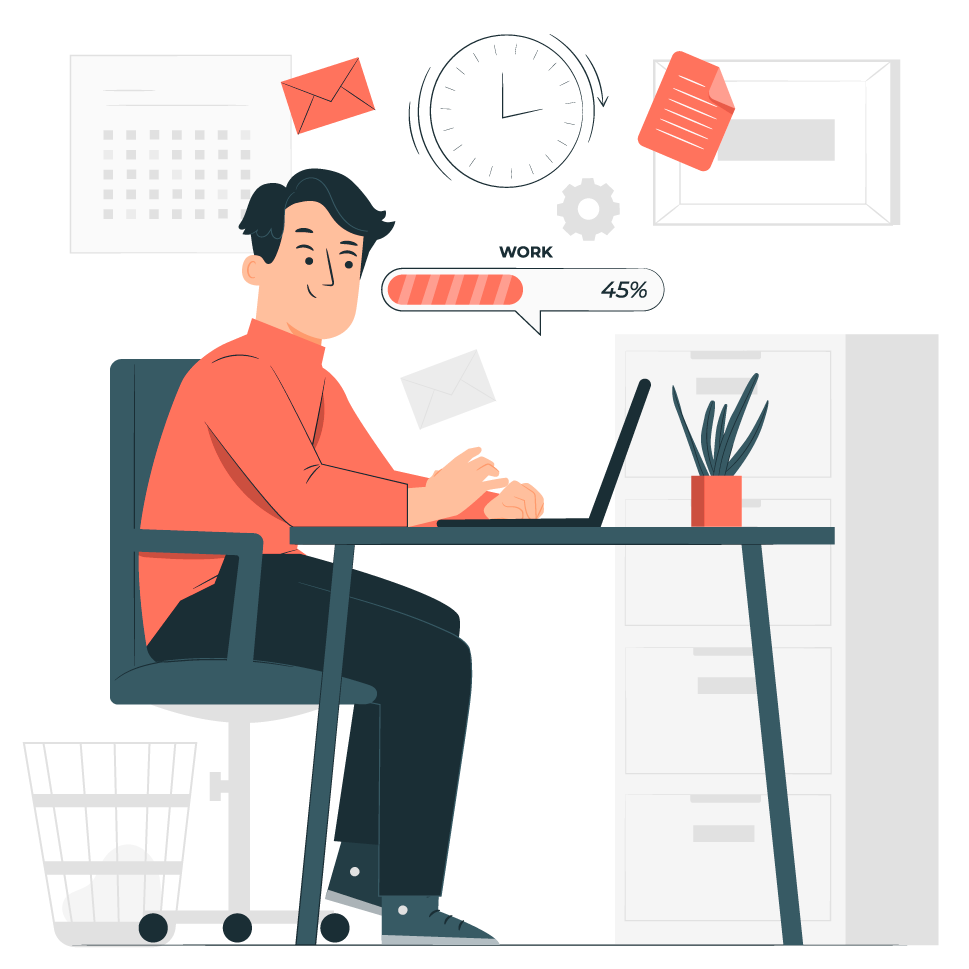
\includegraphics[width=\textwidth]{Imagens/002.ai}
	\footnotesize
	Fonte: elaboração própria (2024) a partir de \textcite{horridge00}
\end{figure}


\subsection{Produção} \label{subsec:producao}

Os setores produtivos seguem os pressupostos neoclássicos de minimização dos custos numa estrutura de mercado de concorrência perfeita, sujeitos a tecnologias de retornos constantes de escala - representadas por funções CES e Leontief. A Figura \ref{fig:estrutura_producao} apresenta a estrutura de produção do modelo. Há cerca de três produtos: 1- bens intermediários; 2- fatores primários; e 3- outros fatores\footnote{"Outros fatores" são as taxas e subsídios do modelo.}. Para se produzir o primeiro, deve-se combinar uma determinada composição das \textit{commodities} disponíveis, decidindo sua origem - se doméstico ou importado. Para produzir o segundo, deve-se combinar quantidades relativas de capital e trabalho, sendo que este é determinado a partir de uma combinação dos três tipos disponíveis de trabalhadores.

Desse modo, para poder produzir nesse modelo, deve-se combinar os bens intermediários, os fatores primários e os outros fatores a partir da minimização dos custos da função Leontief\footnote{Isso implica que esses três fatores são complementares perfeitos, não admitindo substituição}.

\begin{align}
	\underset{i = 1, ... , 124}{Leontief} \{\frac{X_{ij}}{A_{ij}}\} = A_jZ_j, \hspace{2cm} j = 1, ... , 65
\end{align}

No qual $X_{ij}$ corresponde ao insumo $i$ da indústria $j$; $Z_j$ é o nível de atividade da indústria $j$; e $A_ij$ é o coeficiente tecnológico. Se este é igual a 1, significa que é o coeficiente insumo-produto que mostra o insumo mínimo efetivo de $i$ necessário para sustentar uma unidade de atividade na indústria $j$ \cite{dixit80}.

A decisão entre a fonte doméstica ou importada é modelada a partir da hipótese de \textcite{armington69} a qual relaciona os insumos de ambas as fontes como substitutos imperfeitos. Desse modo, para capturar esse efeito, assume-se as unidades de um determinado insumo, diferenciáveis apenas pela fonte, são combinadas para fornecer um só insumo, chamado de \textit{insumo efetivo}:

\begin{align}
	X_{ij} = \underset{s = 1, 2}{CES} = \{\frac{X_{(is)j}}{A_{(is)j}}; \rho_{ij}, b_{(is)j}\}, \hspace{2cm} i & = 1, ... , 124 \\ j & = 1, ... , 65 \notag
\end{align}

No qual $X_{(is)j}$ se refere ao insumo $i$ da fonte $s$ pertencente ao setor $j$; $\rho$ e $b$ são parâmetros de substituição entre as variáveis doméstica e importada. 

\begin{landscape}
	\begin{figure}
		\centering
		\caption{Estrutura de produção do modelo ORANIG-BR} \label{fig:estrutura_producao}
		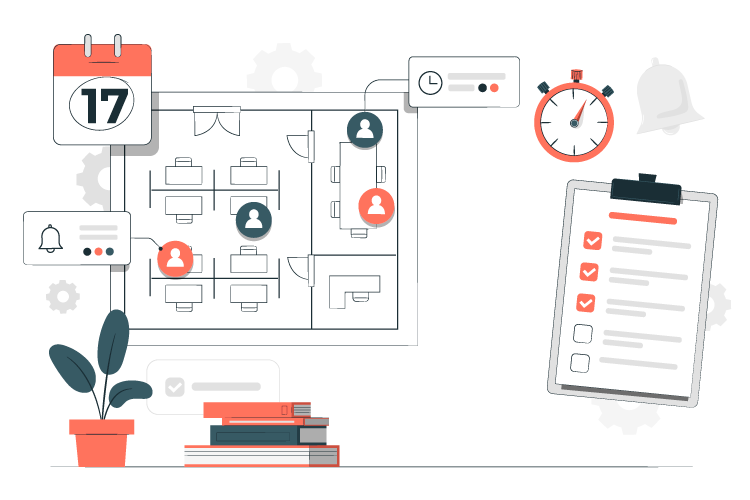
\includegraphics[width=0.9\linewidth]{Imagens/003.ai}
		\footnotesize \\
		Fonte: elaboração própria (2024) a partir de \textcite{horridge00}
	\end{figure}
\end{landscape}

\subsubsection{Composição do fator trabalho} \label{}

Como dito anteriormente, o fator trabalho foi subdividido em três grupos: não qualificado, semi-qualificado e qualificado. Esta divisão segue a intuição de que os produtores buscam um determinado conjunto de habilidades no mercado de trabalho que melhor se adeque a demanda do setor produtivo.

Essa habilidade é representada por anos de educação. O Quadro \ref{quad:categoria_trabalho} apresenta a categorização escolhida para desagregar o fator trabalho.

\begin{quadro}[h]
	\centering
	\begin{threeparttable}
		\caption{Categorização do fator trabalho} \label{quad:categoria_trabalho}
		\footnotesize
		\begin{tabular}{|| m{3cm} | m{9cm} ||}
			\hline \hline
			\multicolumn{1}{||c|}{\textbf{variável}} & \multicolumn{1}{c||}{\textbf{descrição}} \\ \hline
			não qualificado  & até Ensino Fundamental completo (até onze anos de estudo) \\ \hline 
			semi-qualificado & até Ensino Médio completo (doze a quinze anos de estudo) \\ \hline
			qualificado      & Ensino Superior (dezesseis anos ou mais de estudo) \\ \hline \hline
		\end{tabular}
		\begin{tablenotes}
			\scriptsize
			\item Fonte: elaboração própria (2024) a partir do \textcite{inep04}
		\end{tablenotes}
	\end{threeparttable}
\end{quadro}

\subsection{Demanda das famílias} \label{subsec:demanda_familias}

A demanda é composta por cem famílias representativas, distribuídas por percentis da renda total. Cada família determina uma composição ótima de sua cesta de consumo, escolhendo os insumos de tal maneira a maximizar uma função de utilidade Klein-Rubin sujeita a restrição do orçamento familiar \cite{horridge03}. A Figura \ref{fig:estrutura_familia} apresenta a estrutura da demanda das famílias no modelo ORANIG-BR.

A função Klein-Rubin é não-homotética; ou seja, o aumento da renda altera as participações orçamentárias, mesmo com taxas de preço fixas. O consumo é dividido entre dois bens, "subsistência" e "luxo", de tal maneira que o primeiro detém um consumo fixo e o segundo, residual. Diferentemente da função Leontief, a composição das \textit{commodities} é dado por um LES \cite{horridge03}.

Nesse sistema, participação do gasto acima do nível de subsistência, para cada bem, representa uma proporção constante do gasto total de subsistência de cada família representativa. A função de utilidade é dada por:

\begin{align*}
	U(\bar{X}_1, ... , \bar{X}_{124})
\end{align*}

Sujeito a:

\begin{align}
	&\bar{X}_i = \underset{s = 1, 2}{CES} (\bar{X}_{(is)}), \hspace{2cm} i = 1, ... , 124 \\
	&\sum_{s = 1}^{2} \sum_{i = 1}^{124} \bar{P}_{(is)} \bar{X}_{(is)} = C
\end{align}

\begin{landscape}
	\begin{figure}
		\centering
		\caption{Estrutura da demanda das famílias do modelo ORANIG-BR} \label{fig:estrutura_familia}
		\includegraphics[width=0.6\linewidth]{Imagens/004.ai}
		\footnotesize \\
		Fonte: elaboração própria (2024) a partir de \textcite{horridge00}
	\end{figure}
\end{landscape}

\subsection{Fechamento do modelo} \label{subsec:fechamento}

Utiliza-se a versão estática do modelo ORANIG-BR porque as vantagens da dinâmica recursiva não seriam aproveitadas neste exercício empírico. O efeito da estrutura produtiva e da distribuição funcional da renda composição que se espera observar pode ser integralmente captado em um modelo estático.

A Figura~\ref{quad:fechamento} apresenta o fechamento de curto-prazo adotado no modelo, seguindo as especificações de \textcite{horridge03}. Ou seja, tornou-se exógeno: 1- as variáveis do PIB real - exceto a balança comercial; os fatores produtivos; e 3- as taxas de impostos e distribuição dos investimentos entre as indústrias.

Esse fechamento emula o seguinte comportamento econômico. No curto-prazo, o estoque de capital, a tecnologia e o salário real são exógenos. Isso permite ao modelo determinar o emprego real e, consequentemente, o PIB real. Pelo fato do PIB ser determinado pelo lado da oferta, tendo sua absorção doméstica praticamente formada, a balança comercial, no curto-prazo, ganha a função de ser uma variável de ajuste para a identidade do PIB. Ou seja, o movimento do PIB é determinado pelo movimento da balança comercial.

A lista com todas as variáveis exógenas do modelo se encontra no Apêndice~\ref{ap:a}.


\begin{quadro}[h]
	\centering
	\begin{threeparttable}
		\caption{Variáveis de \textit{swap} no fechamento de curto-prazo} \label{quad:fechamento}
		\footnotesize
		\begin{tabular}{||l m{6.5cm} |l m{5.5cm} ||}
			\hline \hline
			\multicolumn{2}{||c|}{\textbf{Antiga exógena}}                     & \multicolumn{2}{c||}{\textbf{Nova exógena}} \\ \hline
			\textbf{Variáveis} & \multicolumn{1}{c|}{\textbf{Descrição}}      & \textbf{Variáveis} & \multicolumn{1}{c||}{\textbf{Descrição}} \\ \hline
			\textit{f1lab\_io}  & mudança geral dos salários                  & \textit{realwage}  & salário real \\
			\textit{x2tot}     & investimento setorial                        & \textit{finv1}     & deslocamento da regra de investimento \\
			\textit{f5tot2}    & desloc. entre demandas do governo e famílias & \textit{x5tot}     & demanda agregada do governo \\
			\textit{invslack}  & var. para tornar o invest. agregado exógeno  & \textit{x2tot\_i}  & investimento agregado por setor \\ \hline \hline
		\end{tabular}
		\begin{tablenotes}
			\scriptsize
			\item Fonte: elaboração própria (2024)
		\end{tablenotes}
	\end{threeparttable}
\end{quadro}


\section{Base de dados e calibragem} \label{sec:dados}

A base de dados do modelo foi calibrada a partir da Matriz de Insumo-Produto do \Citetitle*{scn} do Instituto Brasileiro de Geografia e Estatística (IBGE), contendo 128 produtos e 68 setores econômicos para o ano de 2015. Para esta dissertação, os setores foram agregados em 65 atividades econômicas que produzem 124 produtos. O modelo conta com 114 componentes da demanda final (cem famílias, governo, investimento, exportações e estoque), dois fatores primários (capital e trabalho agregado), três tipos de trabalho (não qualificado, semi-qualificado e qualificado), dois setores de margens (comércio e transporte), e importações por produto para cada um dos 124 produtos.

Para desagregar o fator trabalho e detalhar as famílias em cem classes divididas por percecntis de renda total familiar, utilizou-se, respectivamente, os dados da \Citetitle*{pnad}, do ano de 2015, e da \Citetitle*{pof}, do ano 2008-2009, ambos do IBGE. A escolha por essas edições da PNAD e POF, e não uma mais recente, foi motivada pelo fato do modelo ORANIG-BR ter sido calibrado com os dados desses anos.



\section{Modelo de microssimulação comportamental} \label{sec:microssimulacao}

Como discutido anteriormente, os modelos de equilíbrio geral são utilizados para capturar os efeitos setoriais de variações nos preços relativos e emprego, permitindo focar nos grupos beneficiados e prejudicados a partir de choques exógenos que simulem políticas comerciais, econômicas ou até eventos históricos. Entretanto, não são uma ferramenta adequada para realizar análises distributivas dada a falta de resultados a nível individual \cite{tiberti17}.

Essa limitação está diretamente associada ao pressuposto da Família Representativa\footnote{Nos modelos EGC, o agrupamento familiar é um agregado familiar e não um agregado familiar médio \cite{tiberti17}.} dos modelos de equilíbrio geral. Isso implica que o modelo deve assumir uma distribuição relativa de renda intra-grupo constante para todos - o que não é refletido na realidade. A evidência empírica mostra que componente intra-grupo das mudanças observadas na distribuição de renda é, pelo menos, tão importante quanto o componente entre grupos dessas mudanças \cite{colombo08}.

Por essa razão, os modelos de equilíbrio geral, ao não conseguirem captar esses efeitos a nível microeconômico, podem gerar resultados errôneos - sobretudo se tratando de estudos sobre pobreza. Ao não conseguir capturar a heterogeneidade de uma família, o pressuposto da Família Representativa pode acabar por subestimar o efeito dos choques exógenos \cite{colombo08}. 

Uma alternativa é utilizar os modelos de microssimulação integrados ao modelo de equilíbrio geral. Essa combinação é particularmente útil para estudos sobre desigualdade e pobreza em países em desenvolvimento, uma vez que que tanto o foco micro quanto macroeconômico é requerido: o primeiro para ter um cenário detalhado das rendas e despesas a nível individual, além das reações dos indivíduos frente a choques e outras políticas econômicas; o segundo para poder simular os efeitos diretos e indiretos desses choques sobre toda a estrutura econômica \cite{tiberti17, klevmarken22}.

O modelo de microssimulação pode ser entendido enquanto uma grande variedade de técnicas de modelagem por meio das quais o comportamento ou estado dos indivíduos são estimados ou determinados \cite{figari15}. Na literatura econômica, essa integração macro-micro é amplamente utilizada para avaliar os impactos distributivos de choques e políticas macroeconômicos, particularmente
na área de liberalização comercial \cite{carneiro06, ferreira06, raihan10, cicowiez16, mbanda21}.

Desse modo, para estimar os efeitos do comércio internacional sobre a desigualdade de renda e pobreza ao nível microeconômico, deve-se usar os parâmetros obtidos do modelo de equilíbrio geral em uma nova rodada de microssimulações para investigar os prováveis impactos de choques de demanda de exportação, desvalorização cambial, promoção de exportações, choques de produtividade e liberalização comercial sobre o grau de desigualdade de renda no domicílio e nos níveis de pobreza.

A Figura \ref{fig:microssimulacao} apresenta a estrutura da abordagem do modelo integrado.

\begin{landscape}
	\begin{figure}
		\centering
		\caption{Estrutura esquemática da integração \textit{top-down}} \label{fig:microssimulacao}
		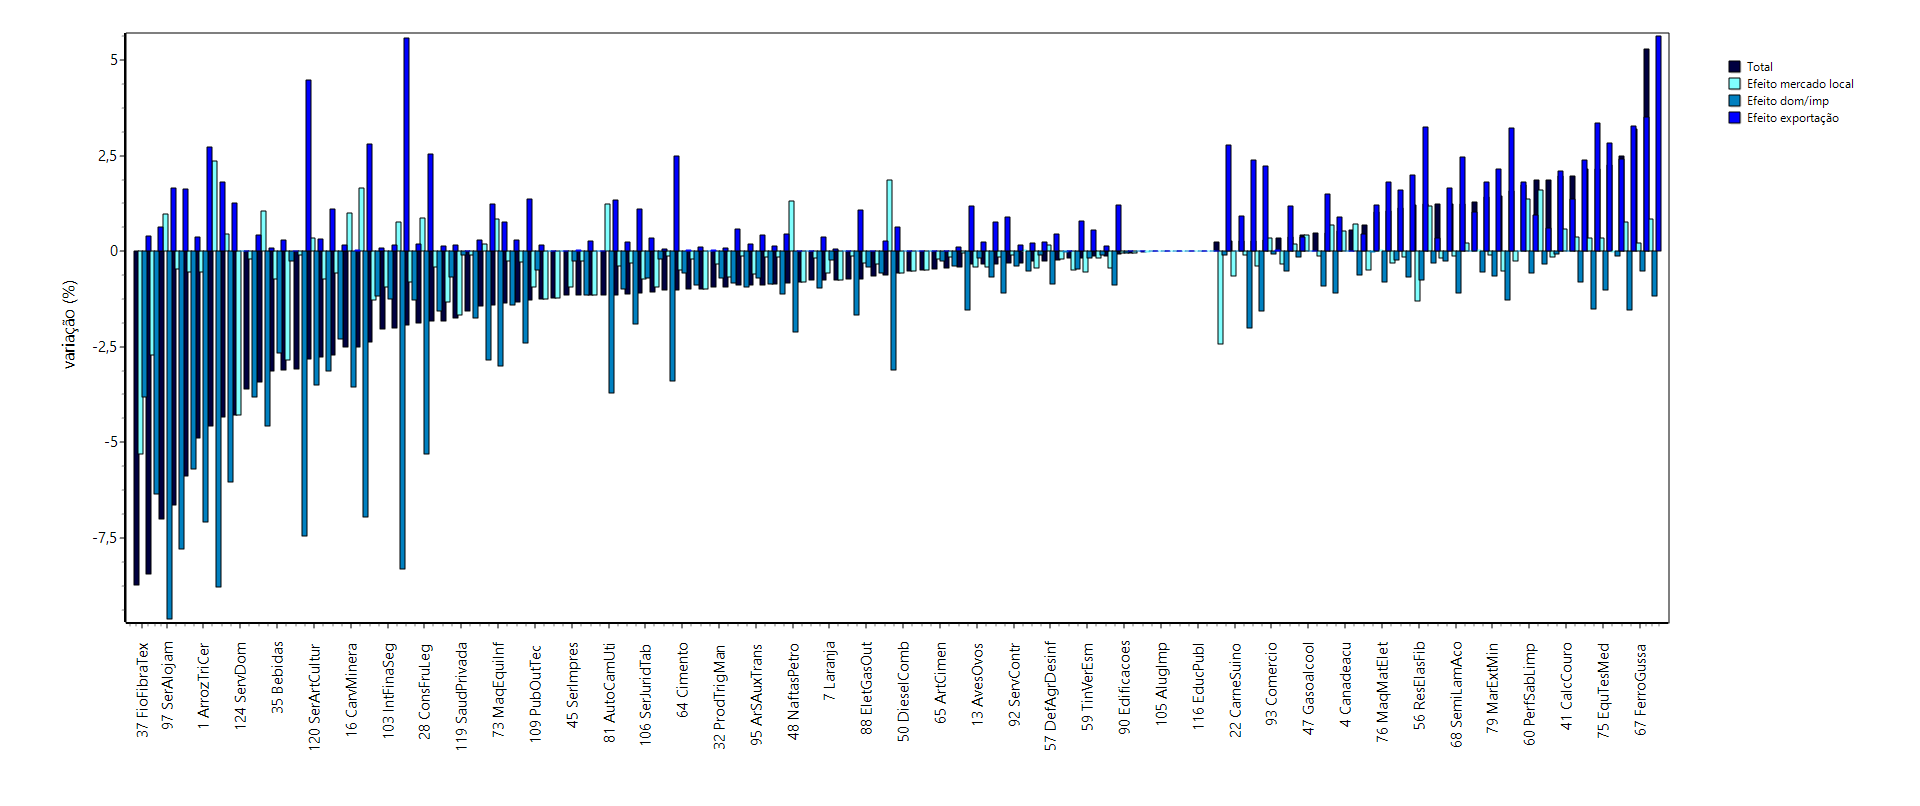
\includegraphics[width=\linewidth]{Imagens/006.ai}
		\footnotesize
		Fonte: elaboração própria (2024)
	\end{figure}
\end{landscape}

\subsection{Forma funcional} \label{subsec:forma_funcional}
 
Baseado na abordagem de \textcite{ganuza07}, utiliza-se dois tipos de microssimulação. O primeiro envolve estimar um modelo de equilíbrio parcial de geração de renda familiar por meio de um sistema de equações que determinam a escolha ocupacional, o retorno do trabalho e do capital humano, os preços ao consumidor e outros componentes da renda familiar e individual. A renda total per capita é definida como:

\begin{align}
	ypc_{hi} = \frac{1}{n_h} \left[ \sum_{i = 1}^{n_h} yp_{hi} + yq_h \right] \label{eq:renda}
\end{align}

No qual:

\vspace{0.5cm}

$
\begin{cases}
	n_h     = \text{tamanho da família $h$;} \\
	yp_{hi} = \text{renda do trabalho do indivíduo $i$ da família $h$} \\
	yq_h    = \text{soma de todas os rendimentos familiares não advindos do trabalho}
\end{cases}
$

\vspace{0.5cm}

E o $yq_h$ é definido como:

\begin{align}
	yq_h = \sum_{i = 1}^{n_h} yqp_{hi} + yqt_h 
\end{align}

No qual:

\vspace{0.5cm}

$
\begin{cases}
	yqp_{hi} = \text{rendimento individual não laboral do membro $i$ da família $h$} \\
	yqt_h    = \text{outras rendas familiares}
\end{cases}
$

\vspace{0.5cm}

A segunda equação é baseada no modelo de \textcite{ganuza02}, conhecida na literatura como \textit{occupational choice model}, estimando a probabilidade do indivíduo permanecer ou ingressar no mercado de trabalho após um determinado choque exógeno.

\begin{align}
	\pi = \pi \left( P, U, S, O, W_1, W_2, M \right) \label{eq:mercado_trabalho}
\end{align}

No qual a estrutura do mercado de trabalho é definido em termos de taxas de participação econômica ($P_j$) e desemprego ($U_j$) entre diferentes grupos $j$ da população em idade ativa definida de acordo com sexo e qualificação, a estrutura de emprego (definido por setor de atividade $S$ e categoria profissional $O$) e remuneração $W_1$, bem como nível global de remuneração $W_2$. A composição de habilidades da população é representada pela variável $M$ \cite{ganuza07}.

\subsection{Abordagem empírica} \label{abordagem_empirica}

A estimação da equação \ref{eq:renda} é realizada através do modelo de duas etapas de Heckman \cite{heckman79} para corrigir o viés de seleção implícito numa regressão de salários\footnote{Só tem salário maior que zero aqueles que estão empregados durante o momento da pesquisa.}. Já a estimação da equação \ref{eq:mercado_trabalho} é feita a partir do estimador de máxima verossimilhança, baseado em \textcite{colombo08}.




% ----------------------------------------------------------
% CAPÍTULO 04 - RESULTADOS
% ----------------------------------------------------------

\chapter{Simulação e Resultados} \label{cha:resultados}

Este capítulo apresenta os resultados da simulação realizada no modelo ORANIG-BR e da microssimulação comportamental para avaliar os efeitos do comércio internacional sobre a desigualdade de renda e pobreza no Brasil. O referido capítulo está dividido em três seções. A primeira descreve a simulação realizada no modelo de equilíbrio geral. A segunda apresenta os resultados do modelo, analisando tanto os efeitos macroeconômicos quanto setoriais, sobre os agentes econômicos, buscando compreender quais foram os grupos beneficiados e prejudicados pela simulação - e a magnitude desse efeito. A terceira e última seção apresenta os resultados do modelo de microssimulação comportamental.



\section{Simulação e mecanismos de transmissão} \label{sec:simulacao}

Propõe-se simular uma política de abertura comercial para avaliar seus efeitos de curto-prazo sobre os indicadores macroeconômicos e setoriais. Essa simulação possibilita mensurar o comportamento das variáveis econômicas frente a uma maior exposição ao comércio internacional, avaliando quais seriam os efeitos de uma política comercial liberalizante.

Por não haver estatísticas mais adequadas para definir a magnitude do choque exógeno desejado neste trabalho, optou-se por realizar uma análise de sensibilidade\footnote{Entende-se por análise de sensibilidade qualquer técnica utilizada para avaliar como variações nas variáveis-chave afetam determinados resultados ou indicadores em um modelo econômico.}. Esse tipo de análise é bastante utilizado na literatura econômica, sobretudo em artigos que buscam mensurar impactos de políticas públicas e acordos comerciais \cite{haddad05, domingues08,perobelli17}. Desse modo, impõe-se aqui uma redução tarifária, por meio do poder da tarifa, no valor de 10\% sobre todas as \textit{commodities} do modelo. Para fins de facilitar a interpretação dos resultados, optou-se por classificar os setores em seis grandes categorias: 1- Agropecuária; 2- Extrativa; 3- Agroindústria; 4- Indústria; 5- Comércio; e 6- Serviços. A descrição completa dessas categorias, bem como os valores utilizados para realizar o choque da simulação, estão disponíveis, respectivamente, no Apêndice~\ref{ap:a} e~\ref{ap:b} deste trabalho.

A Figura~\ref{fig:mecanismos} exibe os mecanismos de transmissão de uma simulação de redução tarifária no modelo ORANIG-BR. Como citado anteriormente, o comércio internacional pode ser entendido enquanto um choque sobre os preços relativos de uma economia. Aqui, isso ocorre através da tarifa de importação: em geral, os bens de uma economia possuem uma tarifa de importação \textit{ad valorem} que afeta diretamente seu preço. Uma mudança sobre essa tarifa torna por alterar o preço do produto. Essa alteração, por conseguinte, varia os preços relativos do produto no mercado mundial.

O efeito esperado é de queda no preço dos produtos e um consequente aumento das importações, uma vez que se tornou mais barato importar. Isso faz com que o produto internacional se torne mais atrativo frente aos produtos do mercado doméstico, havendo uma pressão interna pelo seu consumo. Além disso, pode-se esperar mudança nos retornos dos fatores produtivos dados os novos preços relativos. Como consequência, impõe-se algum nível de reestruturação produtiva a partir dos novos preços e retornos dos fatores produtivos, ajustando-se de acordo com os incentivos.

Sobre as firmas, espera-se um ganho de produtividade das empresas que sejam beneficiadas pela redução tarifária, aumentando sua competitividade no cenário doméstico. Isso fará com que haja uma variação positiva na produção e negativa no índice de preços da economia. Esse novo cenário afeta a renda real de todos os agentes econômicos, beneficiando ou prejudicando os grupos de acordo com a distribuição funcional da renda.

Também é possível esperar um efeito substituição como consequência de uma redução tarifária. Isso pode ocorrer por conta da variação dos preços relativos, que pode tornar mais atrativo importar determinados insumos que consumir sua opção doméstica. Dado esse efeito, espera-se uma variação no produto final, produzido domesticamente, já que houve uma variação no custo de produção. Como último estágio, o efeito substituição gera uma variação na intensidade do comércio internacional, dada a mudança na composição de bens domésticos e importados para produção dos bens nacionais.

Vale a pena ressaltar que também são esperados alguns efeitos \textit{feedback} sempre que haja alteração dos preços e do índice de preços da economia -- que são captados pelo modelo de equilíbrio geral, gerando novas rodadas de efeitos macroeconômicos e setoriais.


\begin{figure}[H]
	\centering
	\caption{Mecanismos de transmissão de uma redução tarifária no modelo ORANIG-BR} \label{fig:mecanismos}
	\includegraphics[width=\textwidth]{Imagens/mecanismos_transmissao.ai}
	\footnotesize
	Fonte: elaboração própria (2024) a partir de \textcite{vinicius18}.
\end{figure}



\section{Resultados do modelo ORANIG-BR} \label{sec:resultados}

A Tabela~\ref{tab:result} apresenta os resultados macroeconômicos do modelo. Percebe-se que a redução tarifária afetou negativamente todos os indicadores de preços, com destaque para o índice preço do consumidor (-0,1156\%), do investimento (-0,1999) e das importações -- que registrou a maior queda: -0,4623\%. A queda conjunta dos preços das exportações e importações incentivaram o aumento da corrente de comércio, sendo liderado pela variação positiva do volume importado (0,1909\%). Esse aumento, largamente composto por insumos voltados à atividade industrial, como apresentado na Tabela~\ref{tab:import}, barateou os custos da produção nacional, resultando em um aumento do emprego real (0,0358\%) e do PIB real (0,0256\%) -- ainda que em valores diminutos. A expansão do volume importado também favoreceu as famílias, que experimentaram um aumendo do consumo real no valor de 0,0555\%.

O deflator do PIB, entendido enquanto um índice de preços implícito que mede a evolução média de preços numa economia, reduziu em 0,1416\%. Esse resultado, em conjunto com o aumento do PIB e emprego real, permite afirmar que a redução tarifária trouxe efeitos positivos sobre os indicadores macroeconômicos, uma vez que se experimentou aumento da atividade econômica e redução dos preços da economia em geral. Entretanto, a variação negativa dos termos de troca (-0,0973), ainda que tímida, aponta que esse cenário não é sustentável, já que as exportações estão perdendo sua capacidade de financiar as importações. 


\begin{table}[h]
	\centering
	\small
	\begin{threeparttable}
		\caption{Efeitos macroeconômicos de curto-prazo da redução tarifária} \label{tab:result}
		\begin{tabular}{m{11cm}c}
			\hline
			\multirow{2}{*}{\textbf{Indicadores}} & \multirow{2}{*}{\textbf{Var. (\%)}} \\
			 &  \\ \hline
			\textbf{Preços} &  \\
			\hspace{0.2cm} Índice de preços do consumidor & -0,1156 \\
			\hspace{0.2cm} Índice de preços do investimento & -0,1999 \\
			\hspace{0.2cm} Índice de preços do governo & -0,1103 \\
			\hspace{0.2cm} Índice de preços das exportações & -0,0973 \\
			\hspace{0.2cm} Índice de preços das importações & -0,4623 \\
			\hspace{0.2cm} Índice de preços do PIB & -0,1416 \\
			\hspace{0.2cm} Termos de troca & -0,0973 \\
			\hspace{0.2cm} Custos dos fatores primários & -0,0617 \\
			\hspace{0.2cm} Salário nominal & -0,1156 \\
			\hspace{0.2cm} Desvalorização real & 0,1418 \\ \hline
			\textbf{Volume} &  \\
			\hspace{0.2cm} Consumo real das famílias & 0,0555 \\
			\hspace{0.2cm} Volume exportado & 0,1009 \\
			\hspace{0.2cm} Volume importado & 0,1909 \\
			\hspace{0.2cm} PIB real & 0,0256 \\
			\hspace{0.2cm} Emprego real & 0,0358 \\ \hline
		\end{tabular}
	\begin{tablenotes}
		\footnotesize
		\item Fonte: elaboração própria (2024) com base nas simulações feitas no ORANIG-BR.
	\end{tablenotes}
	\end{threeparttable}
\end{table}

A Tabela~\ref{tab:ativ} apresenta os resultados setoriais da redução tarifária sobre o nível de atividade econômica e emprego, selecionando os dez setores produtivos com as maiores e menores variações percentuais no nível de atividade. As correspondências dos setores estão disponíveis no Apêndice~\ref{ap:a}.

Os setores mais beneficiados foram aqueles que utilizam os insumos importados que tiveram as maiores reduções em seus preços de importações. Foi o caso do setor de Fabricação de calçados e de artefatos de couro (C15) que experimentou a maior variação no nível de atividade econômica (0,1849\%) e emprego (0,2483\%). Como apresentado na Tabela~\ref{tab:import}, a \textit{commodity} Tecido (C38) foi a que registrou a maior variação negativa em seu preço de importação e, por conseguinte, maior variação positiva em seu volume importado. Essa \textit{commodity} representa, sozinha, quase 20\% dos produtos importados pelo setor de Fabricação de calçados. Desse modo, a redução tarifária funcionou como um corte de custos de produção, permitindo expandir seu nível de produção e emprego.

É possível notar que as maiores variações positivas não se concentraram em nenhum dos setores agregados: quatro desses seis grandes setores estão entre aqueles com maior expansão do nível de atividade econômica. Entretanto, as maiores variações negativas estão concentradas no setor industrial, com destaque para Fabricação de produtos têxteis (C13) que registrou a maior retração de sua atividade econômica (-0,6101\%) e emprego (-0,7916\%). Essa concentração no setor industrial é explicada pela perda de competitividade desses setores frente a uma maior abertura comercial. Ou seja, a redução tarifária reduziu o \textit{market share} desses setores na economia doméstica. A Tabela~\ref{tab:fandecomp} apresenta os dados que corroboram essa afirmação, sendo discutida em detalhes mais abaixo.


\begin{table}[h]
	\centering
	\small
	\begin{threeparttable}
		\caption{Efeitos de curto-prazo da redução tarifária sobre o nível de atividade e emprego (var. \%)}\label{tab:ativ}
		\begin{tabular}{m{2cm} >{\centering\arraybackslash}m{4cm} >{\centering\arraybackslash}m{4cm} >{\centering\arraybackslash}m{4cm} >{\centering\arraybackslash}m{4cm}}
			\hline
			\multirow{2}{*}{\textbf{Setores}} & \multirow{2}{*}{\textbf{Setores agregados}} & \multicolumn{2}{c}{\textbf{Indicadores}} \\ \cline{3-4} &  & \textbf{Nível de atividade} & \textbf{Emprego} \\ \hline
			C15 & Indústria     & 0,1849  & 0,2483 \\
			C35 & Indústria     & 0,1148  & 0,1379 \\
			C44 & Serviços      & 0,0809  & 0,1079 \\
			C37 & Serviços      & 0,0802  & 0,1472 \\
			C07 & Extrativa     & 0,0743  & 0,1413 \\
			C65 & Serviços      & 0,0661  & 0,0661 \\
			C60 & Serviços      & 0,0636  & 0,0690 \\
			C23 & Indústria     & 0,0618  & 0,0891 \\
			C62 & Serviços      & 0,0531  & 0,1027 \\
			C12 & Agroindústria & 0,0489  & 0,1476 \\ \hline
			C13 & Indústria     & -0,6101 & -0,7916 \\
			C14 & Indústria     & -0,1955 & -0,2686 \\
			C25 & Indústria     & -0,1342 & -0,1652 \\
			C36 & Indústria     & -0,1041 & -0,1985 \\
			C29 & Indústria     & -0,0368 & -0,0543 \\
			C33 & Indústria     & -0,0279 & -0,0298 \\
			C26 & Indústria     & -0,0251 & -0,0339 \\
			C16 & Indústria     & -0,0193 & -0,0314 \\
			C21 & Indústria     & -0,0099 & -0,0215 \\
			C27 & Indústria     & -0,0085 & -0,0149 \\ \hline
			\end{tabular}
		\begin{tablenotes}
			\footnotesize
			\item Fonte: elaboração própria (2024) com base nas simulações feitas no ORANIG-BR.
		\end{tablenotes}
		\end{threeparttable}
\end{table}

A Tabela~\ref{tab:fandecomp} apresenta a decomposição dos efeitos de curto-prazo da redução tarifária em quatro categorias: 1- Mercado Local; 2- Substituição; 3- Exportação; e 4- Total. A primeira deve ser entendida enquanto o nível de produção esperado dado uma mudança na demanda interna do produto, independentemente da fonte -- se doméstico ou importado. A segunda pode ser interpretada como o valor pelo qual a produção dos bens nacionais varia devido a uma mudança relativa de preços que favoreça a substituição de importações. A terceira mostra a contribuição da variação das exportações para a variação da produção nacional. A quarta e última coluna é a soma dos valores das três outras categorias.

O efeito Mercado Local foi o responsável pelas maiores variações positivas do efeito Total. Dentre essas, destacam-se as \textit{commodities} mais relacionadas com a Indústria: Calçados e artefatos de couro (C41), Aeronaves, embarcações e outros equipamentos de transporte (C84) e Eletrodomésticos (C77). Isso significa que a produção desses bens teria que ter aumentado na magnitude do efeito Mercado Local para poder ter atendido a pressão sobre a demanda realizada pelo corte tarifário.

Por outro lado, o efeito Substituição foi dominante nas maiores variações negativas do efeito Total. Isso significa que esses produtos perderam competitividade no mercado doméstico frente a uma maior exposição ao mercado internacional. Dentre esses, pode-se destacar as \textit{commodities} Tecido (C38), Fios e fibras têxteis beneficiadas (C37) e Art. têxteis de uso doméstico e outros têxteis (C39).

Desse modo, pode-se afirmar que a indústria foi o setor agregado mais afetado pela redução tarifária, havendo uma parcela de si por ela beneficiada -- como, por exemplo, os setores voltados para a fabricação de couro e calçado -- e outra parcela por ela prejudicada -- neste caso, os setores voltados para a fabricação têxtil. Como expõe a Tabela~\ref{tab:ativ}, os setores relacionados com Serviços, Extrativa e Agroindústria também foram beneficiados pela abertura comercial, entretanto, gozando de um ganho mais diminuto.


\begin{table}[H]
	\centering
	\small
	\begin{threeparttable}
		\caption{Decomposição dos efeitos de curto-prazo da redução tarifária (var. \%)} \label{tab:fandecomp}
		\begin{tabular}{lccccc}
		\hline
		\multirow{2}{*}{\textit{\textbf{Commodities}}} &
		\multicolumn{1}{c}{\multirow{2}{*}{\textbf{Setores agregados}}} &
		\multicolumn{4}{c}{\textbf{Efeitos}} \\ \cline{3-6} 
		&
		\multicolumn{1}{c}{} &
		\multicolumn{1}{c}{\textbf{Mercado local}} &
		\multicolumn{1}{c}{\textbf{Substituição}} &
		\multicolumn{1}{c}{\textbf{Exportação}} &
		\multicolumn{1}{c}{\textbf{Total}} \\ \hline
		C41  &	Indústria	  &	 0,1275	&  0,0001 &	0,0514	&  0,1790	\\	
        C84  &	Indústria	  &	 0,0323	&  -0,006 &	0,0846	&  0,1109	\\	
		C77  &	Indústria	  &	 0,0974	&  -0,024 &	0,0053	&  0,0788	\\	
		C97  &	Serviços	  &	 0,0189	&  0,0354 &	0,0240	&  0,0783	\\	
		C72  &	Indústria	  &	 0,0326	&  0,0059 &	0,0388	&  0,0774	\\	
		C20  &	Extrativa	  &	 0,0173	&  0,0057 &	0,0461	&  0,0691	\\	
		C124 &	Serviços	  &	 0,0661	&  0      &	0	    &  0,0661	\\	
		C79  &	Indústria	  &	 0,0093	& -0,0061 &	0,0610	&  0,0643	\\	
		C87  & 	Serviços	  &	 0,0149	&  0,0424 &	0,0068	&  0,0641	\\	
		C117 & 	Serviços	  &	 0,0608	&  0,0009 &	0,0001	&  0,0618	\\	\hline
		C38  & 	Indústria	  &	-0,1082	& -0,6980 &	0,0412	& -0,7650	\\	
		C37  &	Indústria	  &	-0,3986	& -0,2799 &	0,0189	& -0,6596	\\	
		C39  & 	Indústria	  &	-0,0042	& -0,4037 &	0,0054	& -0,4025	\\	
		C86  &	Indústria	  &	 0,0897	& -0,3485 &	0,0502	& -0,2086	\\	
		C40  &	Indústria	  &	 0,2318	& -0,4374 &	0,0057	& -0,1999	\\	
		C62  &	Indústria	  &	 0,0319	& -0,3109 &	0,1234	& -0,1556	\\	
		C63  &	Indústria	  &	-0,0032	& -0,1508 &	0,0261	& -0,1279	\\	
		C03  &	Agropecuária  &	-0,1934	& -0,0012 &	0,1318	& -0,0627	\\	
		C56  &	Indústria	  &	-0,0772	& -0,0322 &	0,0521	& -0,0574	\\	
		C24  &	Agroindústria &	 0,0705	& -0,1505 &	0,0276	& -0,0524	\\	\hline

		\end{tabular}
	\begin{tablenotes}
		\footnotesize
		\item Fonte: elaboração própria (2024) com base nas simulações feitas no ORANIG-BR.
	\end{tablenotes}
	\end{threeparttable}
\end{table}


A Tabela~\ref{tab:import} exibe os efeitos de curto-prazo da redução tarifária sobre o volume e preço das importações por \textit{commodity}. A maior exposição ao mercado internacional aumentou a demanda pelos produtos dos setores da Indústria, Agroindústria e Agropecuária. Como citado anteriormente, a expansão nas importações desses produtos, em especial Tecido (C38), Artigos do vestuário e acessórios (C40) e Artigos têxteis de uso doméstico e outros têxteis (C39), é resultado da redução dos custos de produção proporcionada pelo corte tarifário, que tornou por baixar o preço de importação desses bens. Os menores preços permitiram uma expansão no nível de atividade e emprego dos setores que tem esses bens como insumos.

A segunda metade da Tabela apresenta as \textit{commodities} com as maiores variações negativas de volume importado. Isso ocorre pois esses bens já não contavam com nenhuma barreira tarifária, logo, seus preços de importações não foram afetados pelo corte tarifário. O volume importado tornou por reduzir por conta da mudança dos preços relativos que pressionaram a demanda por importações de outros produtos, esses sim, afetados pelo corte tarifário.


\begin{table}[h]
	\centering
	\small
	\begin{threeparttable}
		\caption{Efeitos de curto-prazo da redução tarifária sobre as importações (var. \%)} \label{tab:import}
		\begin{tabular}{m{3cm} >{\centering\arraybackslash}m{3cm} >{\centering\arraybackslash}m{3cm} >{\centering\arraybackslash}m{3cm}}
			\hline
			\multirow{2}{*}{\textit{\textbf{Commodities}}} & \multirow{2}{*}{\textbf{Setores agregados}} & \multicolumn{2}{c}{\textbf{Importações}} \\ \cline{3-4} 
			      &               & \textbf{Volume} & \textbf{Preço} \\ \hline
			 C38  & Indústria     &  2,7413         & -2,6082 \\
			 C40  & Indústria     &  2,6257         & -2,4429 \\
			 C39  & Indústria     &  1,9852         & -1,6339 \\
			 C27  & Agroindústria &  1,4747         & -0,5882 \\
			 C42  & Indústria     &  1,4279         & -0,8667 \\
			 C6   & Agropecuária  &  1,2962         & -0,9169 \\
			 C34  & Agroindústria &  1,2562         & -1,1298 \\
			 C63  & Indústria     &  1,2292         & -1,1688 \\
			 C37  & Agroindústria &  1,2211         & -1,7473 \\ \hline
			 C90  & Serviços      & -0,1760         & 0       \\
			 C87  & Serviços      & -0,1648         & 0       \\
			 C92  & Serviços      & -0,1412         & 0       \\
			 C102 & Serviços      & -0,0953         & 0       \\
			 C96  & Comércio      & -0,0925         & 0       \\
			 C111 & Serviços      & -0,0891         & 0       \\
			 C112 & Serviços      & -0,0868         & 0       \\
			 C23  & Extrativa     & -0,0798         & 0       \\
			 C94  & Serviços      & -0,0618         & 0       \\ \hline
			\end{tabular}
		\begin{tablenotes}
			\footnotesize
			\item Fonte: elaboração própria (2024) com base nas simulações feitas no ORANIG-BR.
		\end{tablenotes}
		\end{threeparttable}
\end{table}

A literatura econômica afirma que o comércio internacional gera ganhadores e perdedores. Os resultados do modelo ORANIG-BR indicam que uma redução tarifária beneficiaria os setores da Agroindústria, Agropecuária e uma parte da Indústria -- mais relacionada com produção de tecidos e calçados. Por outro lado, haveria perda de \textit{market share} de uma outra parcela industrial brasileira, mais relacionada com a produção têxtil, reduzindo, por conseguinte, seu nível de atividade econômica. Entretanto, os indicadores macroeconômicos sugerem que os ganhos do primeiro grupo foram capazes de superar as perdas do segundo grupo, levando a uma redução dos preços da economia e um aumento do PIB real, emprego agregado e consumo das famílias.



\section{Resultados da microssimulação comportamental} \label{sec:microssimulacao}

Os resultados do modelo de geração da renda familiar estão expostos na Tabela~\ref{tab:result_microssimulacao}. Como descrito na subseção~\ref{subsec:integracao}, após estimar o cenário \textit{benchmarking} da microssimulação, usa-se os parâmetros de emprego e salários, obtidos no modelo ORANIG-BR, para estimar uma nova rodada de microssimulação, aqui chamada de cenário integração. Os índices de Gini e FGT são calculados em cima desses dois cenários, observando a variação desses indicadores entre o benchmarking e integração -- que expressa os efeitos do choque exógeno sobre a desigualdade de renda e pobreza.

Os coeficientes da Correção de Heckman e da escolha ocupacional, bem como os resultados do cenário \textit{benchmarking} e os parâmetros de variação de salário e emprego estão disponíveis no Apêndice~\ref{ap:b}.

\begin{table}[h]
	\centering
	\small
	\begin{threeparttable}
		\caption{Microssimulação dos efeitos da redução tarifária sobre desigualdade de renda e pobreza por qualificação} \label{tab:result_microssimulacao}
		\begin{tabular}{m{8cm} >{\centering\arraybackslash}m{2cm} >{\centering\arraybackslash}m{2cm}}
			\hline
			\multirow{2}{*}{}                     & \multirow{2}{*}{\textbf{Simulado}} & \multirow{2}{*}{\textbf{Variação (\%)}} \\
			                                      &                           &                                \\ \hline
			\textbf{Pobreza$^{\dag}$}             &                           &                                \\
			\hspace{0.2cm} $\text{FGT}_0$         & 31,39                     & 0,024                          \\
			\hspace{0.2cm} $\text{FGT}_1$         & 14,34                     & 0,013                          \\
			\hspace{0.2cm} $\text{FGT}_2$         & 9,02                      & 0,010                          \\ \hline
			\textbf{Extrema pobreza$^{\ddagger}$} &                           &                                \\
			\hspace{0.2cm} $\text{FGT}_0$         & 8,64                      & --                             \\
			\hspace{0.2cm} $\text{FGT}_1$         & 4,30                      & 0,004                          \\
			\hspace{0.2cm} $\text{FGT}_2$         & 2,87                      & 0,003                          \\ \hline
			\textbf{Desigualdade de renda}        &                           &                                \\
			\hspace{0.2cm} Gini                   & 0,521                     & -0,007                         \\ \hline
			\end{tabular}
	\begin{tablenotes}
		\footnotesize
		\item Fonte: elaboração própria (2024) com base nos dados da PNAD 2015.
		\item \textit{Nota:}
		\item \hspace{0.2cm} $^{\dag}$     Indivíduos com renda familiar per capita abaixo de R\$367,02.
		\item \hspace{0.2cm} $^{\ddagger}$ Indivíduos com renda familiar per capita abaixo de R\$126,79.
	\end{tablenotes}
	\end{threeparttable}
\end{table}

Os resultados apontam que o potencial da abertura comercial para afetar a desigualdade de renda e pobreza é praticamente nulo, uma vez que seus índices variaram muito pouco. Mesmo assim, observou-se uma redução na desigualdade de renda e elevação dos níveis de pobreza e pobreza extrema.

As maiores variações foram na proporção de pobres (0,024\%), na intensidade (0,013\%) e na severidade da pobreza (0,010\%). Ou seja, a redução das tarifas de importação brasileiras gerou um aumento no quantitativo de pobres e os distanciou da linha de pobreza -- entretanto, numa ínfima magnitude. 

Não se registrou variação na proporção de pobres para a pobreza extrema, mantendo-se estável frente a redução tarifária. Experimentou-se uma diminuta elevação na intensidade (0,004\%) e severidade da pobreza (0,003\%); entretanto, sem nenhum expressividade.

Analisando o índice de Gini, percebe-se o efeito contrário. A redução tarifária engendrou uma redução na desigualdade de renda (-0,007\%). Apesar da variação ínfima, é interessante destacar a direção contrária dos efeitos de desigualdade e pobreza observados.

Desse modo, pode-se afirmar que, de acordo com os resultados da microssimulação, uma redução tarifária no montante de 10\% levou ao aumento da pobreza absoluta e extrema, ao passo em que se observou uma redução dos níveis de desigualdade de renda. Para além disso, a microssimulação também constatou que o comércio internacional tem um potencial bastante limitado para afetar esses indicadores de maneira expressiva, sobretudo os indicadores de pobreza extrema e de desigualdade.

Existem diversas evidências na literatura econômica que convergem para os resultados aqui encontrados. Tanto sobre a diminuta influência do comércio internacional \cite{carneiro06} quanto sobre os resultados divergentes entre desigualdade de renda e pobreza \cite{borrazetal12}.

Por fim, várias razões podem explicar o comportamento dos indicadores de desigualdade de renda e pobreza encontrados. Sobre a diminuta influência, uma das razões pode ser que as barreiras tarifárias já não sejam altas o suficiente para que uma nova redução traga efeitos expressivos.

Uma possível razão que explique o generalizado aumento da pobreza absoluta e extrema, ainda que parco, pode estar relacionado a estrutura produtiva brasileira e seu perfil de pauta exportadora. Como vimos anteriormente, a redução tarifária afetou proporcionalmente os setores da Agroindústria, pouco intensiva em trabalho, e prejudicando os setores industriais de produção têxtil, comparativamente mais intensivos em trabalho. Essa distribuição, somada a uma redução do salário nominal em 0,11\%, pode explicar o aumento da pobreza. Entretanto, não é possível testar quaisquer dessas suposições com a estratégia empírica aqui utilizada, deixando essas questões a serem exploradas em trabalhos futuros.




% ----------------------------------------------------------
% CAPÍTULO 05 - CONSIDERAÇÕES FINAIS
% ----------------------------------------------------------

\chapter{Considerações finais}

Este trabalho tem como objetivo estimar os efeitos do comércio internacional sobre a distribuição da renda familiar e sobre os indicadores de pobreza no Brasil. Para isso, optou-se por utilizar um modelo nacional de equilíbrio geral computável integrado uma abordagem de microssimulações comportamentais que permite, em conjunto, avaliar os resultados tanto a nível macroeconômico quanto microeconômico.

Como simulação, foi proposto uma redução tarifária no montante de 10\% sobre todas as \textit{commodities} da economia para observar os efeitos de curto-prazo de uma política orientada para a liberalização comercial. Os resultados macroeconômicos apontaram para ganhos nos setores da Agroindústria e parte da Indústria, mais voltada para o setor de tecidos e calçados -- pouco intensivos em trabalho -- ao passo em que se registrou perdas para boa parte da Indústria, especialmente os setores têxteis. Também se observou que os ganhos foram grandes o suficiente para superar as perdas, uma vez que houve aumento do PIB real, emprego agregado e consumo das famílias.

Entretanto, essa maior exposição ao comércio internacional não promoveu melhorias e tampouco deteriorações nos indicadores de desigualdade de renda. O mesmo pode ser dito para os indicadores de pobreza no Brasil. As variações observadas nos índices de Gini e FGT foram bastante modestas, sobretudo quando se trata de extrema pobreza e desigualdade de renda, no qual a influência do comércio internacional foi praticamente nula. Isso converge para os resultados de \textcite{carneiro06}: liberalizações comerciais são pouco eficazes para influenciar esses indicadores.

Mesmo assim, apesar do diminuto efeito, o modelo de microssimulação comportamental registrou aumento generalizado nos indicadores de pobreza absoluta e extrema para as três categorias de qualificação, havendo sua maior variação na proporção dos extremamente pobres entre os não qualificados e dos pobres entre os semi-qualificados e qualificados, além de haver uma expansão do \textit{gap} da pobreza para os semi-qualificados. Sobre a desigualdade de renda, a direção do efeito foi contrária: observou-se uma redução para os três grupos. A direção desses resultados converge com as evidências encontradas por \textcite{borrazetal12}.

Por fim, várias razões podem explicar esses resultados. Apesar de não ser possível testá-las neste trabalho, uma possível explicação para a diminuta influência do comércio internacional esteja ancorada no fato em que as barreiras tarifárias brasileiras já não sejam altas o suficiente para que uma redução gere resultados expressivos. Sobre os efeitos divergentes da desigualdade de renda e pobreza, uma possível explicação esteja na estrutura produtiva brasileira, no qual a redução tarifária prejudicou os setores comparativamente mais intensivos em trabalho, gerando, como consequência, elevação dos níveis de pobreza.






% ----------------------------------------------------------
% ELEMENTOS PÓS-TEXTUAIS
% ----------------------------------------------------------
\postextual

% Referências:
\begingroup
\printbibliography[title = Referências, heading = bibintoc, notkeyword = {consulta}, notkeyword={npub-informal}]
\endgroup

% Capítulos pós-textuais:
%\addtocontents{toc}{\vspace{4pt}}

% Apêndice:

%---------------------------------------------------------------------
% APÊNDICE
%---------------------------------------------------------------------

\begin{apendicesenv}
	%\renewcommand{\thechapter}{\arabic{chapter}}
	\partapendices
	\chapter{Tabela de dados} \label{ap:a}

	\begin{small}
		\begin{center}
			\begin{longtable}{m{8cm}ccc}
				\caption{Redução tarifária para as \textit{commodities} do modelo ORANIG-BR}\label{ap:choque} \\
				
				\hline
				\multirow{2}{*}{\textit{\textbf{Commodities}}} & \multirow{2}{*}{\textbf{\thead{Redução tarifária \\ (-10\%)}}} & \multicolumn{2}{c}{\textbf{Tarifa de importação}} \\ \cline{3-4} 
				&  & \multicolumn{1}{c}{\textbf{Antes}} & \multicolumn{1}{c}{\textbf{Depois}} \\ \hline \endfirsthead

				\multicolumn{4}{c}{{\bfseries \tablename\ \thetable{} -- continuação da página anterior}} \\
				\hline
				\multirow{2}{*}{\textit{\textbf{Commodities}}} & \multirow{2}{*}{\textbf{\thead{Redução tarifária \\ (-10\%)}}} & \multicolumn{2}{c}{\textbf{Tarifa de importação}} \\ \cline{3-4} 
				&  & \multicolumn{1}{c}{\textbf{Antes}} & \multicolumn{1}{c}{\textbf{Depois}} \\ \hline \endhead

				\hline \multicolumn{4}{r}{{Continua na próxima página}} \\ \hline
				\endfoot

				\hline \endlastfoot

				Arroz, trigo e outros cereais                      & -0,08935 & 0,009016 & 0,008114 \\
				Milho em grão                                      & 0 & 0 & 0 \\
				Algodão herbáceo, outras fibras da lav. temp.      & -0,55556 & 0,058824 & 0,052942 \\
				Cana-de-açúcar                                     & 0 & 0 & 0 \\
				Soja  em grão                                      & 0 & 0 & 0 \\
				Outros produtos e serviços da lavoura temp.        & -0,91687 & 0,100942 & 0,090848 \\
				Laranja                                            & -0,76923 & 0,083333 & 0,075000 \\
				Café em grão                                       & 0 & 0 & 0 \\
				Outros produtos da lavoura permanente              & -0,57036 & 0,060486 & 0,054437 \\
				Bovinos e outros animais vivos                     & 0 & 0 & 0 \\
				Leite de vaca e de outros animais                  & 0 & 0 & 0 \\
				Suínos                                             & 0 & 0 & 0 \\
				Aves e ovos                                        & 0 & 0 & 0 \\
				Produtos da exploração florestal e da silvicultura & -0,36942 & 0,038359 & 0,034523 \\
				Pesca e aquicultura                                & -0,02209 & 0,002214 & 0,001993 \\
				Carvão mineral                                     & 0 & 0 & 0 \\
				Minerais não-metálicos                             & -0,08734 & 0,008811 & 0,007930 \\
				Petróleo, gás natural e   serviços de apoio        & 0 & 0 & 0 \\
				Minério de ferro                                   & 0 & 0 & 0 \\
				Minerais metálicos não-ferrosos                    & -0,01124 & 0,001125 & 0,001013 \\
				Carne de bovinos e outros   prod. de carne         & -0,26071 & 0,026769 & 0,024092 \\
				Carne de suíno                                     & 0 & 0 & 0 \\
				Carne de aves                                      & 0 & 0 & 0 \\
				Pescado industrializado                            & -0,468 & 0,049098 & 0,044188 \\
				Leite resfriado, esterilizado   e pasteurizado     & 0 & 0 & 0 \\
				Outros produtos do laticínio                       & -0,40385 & 0,042084 & 0,037876 \\
				Açúcar                                             & -0,58824 & 0,062500 & 0,056250 \\
				Conservas de frutas, legumes, outros vegetais      & -0,61502 & 0,065532 & 0,058979 \\
				Óleos e gorduras vegetais e animais                & -0,6536 & 0,069931 & 0,062938 \\
				Café beneficiado                                   & -0,63569 & 0,067884 & 0,061096 \\
				Arroz beneficiado e produtos derivados do arroz    & -0,08699 & 0,008775 & 0,007898 \\
				Produtos derivados do trigo, mandioca ou milho     & -0,42956 & 0,044884 & 0,040396 \\
				Rações balanceadas para animais                    & -0,69753 & 0,074983 & 0,067485 \\
				Outros produtos alimentares                        & -1,12976 & 0,127365 & 0,114629 \\
				Bebidas                                            & -0,37518 & 0,038980 & 0,035082 \\
				Produtos do fumo                                   & -0,01575 & 0,001577 & 0,001419 \\
				Fios e fibras têxteis   beneficiadas               & -1,74727 & 0,211720 & 0,190548 \\
				Tecidos                                            & -2,60817 & 0,352845 & 0,317561 \\
				Art. têxteis de uso doméstico   e outros têxteis   & -1,63393 & 0,195305 & 0,175775 \\
				Artigos do vestuário e acessórios                  & -2,44292 & 0,323263 & 0,290937 \\
				Calçados e artefatos de couro                      & -2,92959 & 0,414346 & 0,372911 \\
				Produtos de madeira, exclusive móveis              & -0,86667 & 0,094891 & 0,085402 \\
				Celulose                                           & -0,24014 & 0,024605 & 0,022145 \\
				Papel, papelão, embalagens e artefatos de papel    & -0,66523 & 0,071264 & 0,064138 \\
				Serviços de impressão e reprodução                 & -0,54054 & 0,057143 & 0,051429 \\
				Combustíveis para aviação                          & 0 & 0 & 0 \\
				Gasoálcool                                         & 0 & 0 & 0 \\
				Naftas para petroquímica                           & 0 & 0 & 0 \\
				Óleo combustível                                   & 0 & 0 & 0 \\
				Diesel - biodiesel                                 & 0 & 0 & 0 \\
				Outros produtos do refino do petróleo              & -0,01265 & 0,001267 & 0,001140 \\
				Etanol e outros   biocombustíveis                  & -0,18155 & 0,018491 & 0,016642 \\
				Produtos químicos inorgânicos                      & -0,10249 & 0,010355 & 0,009320 \\
				Adubos e fertilizantes                             & -0,09772 & 0,009868 & 0,008881 \\
				Produtos químicos orgânicos                        & -0,38194 & 0,039711 & 0,035740 \\
				Resinas,elastômeros e fibras artif. e sintéticas   & -0,88012 & 0,096505 & 0,086855 \\
				Defensivos agrícolas e desinfestantes              & -0,30735 & 0,031710 & 0,028539 \\
				Produtos químicos diversos                         & -0,71111 & 0,076555 & 0,068900 \\
				Tintas, vernizes, esmaltes e lacas                 & -1,22347 & 0,139403 & 0,125463 \\
				Perfumaria, sabões e artigos de limpeza            & -0,29736 & 0,030647 & 0,027582 \\
				Produtos farmacêuticos                             & -0,33044 & 0,034173 & 0,030756 \\
				Artigos de borracha                                & -1,074 & 0,120322 & 0,108290 \\
				Artigos de plástico                                & -1,16882 & 0,132352 & 0,119117 \\
				Cimento                                            & -0,31708 & 0,032746 & 0,029471 \\
				Artefatos de cimento, gesso e semelhantes          & -0,90909 & 0,100000 & 0,090000 \\
				Vidros, cerâmicos e outros prod. de minerais       & -0,89687 & 0,098523 & 0,088671 \\
				Ferro-gusa e ferroligas                            & -0,43596 & 0,045583 & 0,041025 \\
				Semi-acabados, laminados planos e tubos            & -0,90836 & 0,099912 & 0,089921 \\
				Produtos da metalurgia de metais não-ferrosos      & -0,18425 & 0,018771 & 0,016894 \\
				Peças fundidas de aço e de metais não ferrosos     & 0 & 0 & 0 \\
				Produtos de metal, excl. máquinas e equip.         & -1,29002 & 0,148108 & 0,133297 \\
				Componentes eletrônicos                            & -0,16212 & 0,016479 & 0,014831 \\
				Máquinas para escritório e equip. de informática   & -0,43944 & 0,045964 & 0,041368 \\
				Material eletrônico e equip. de comunicações       & -0,61592 & 0,065635 & 0,059072 \\
				Equip. de medida, teste e controle                 & -0,68245 & 0,073244 & 0,065920 \\
				Máquinas, aparelhos e materiais elétricos          & -1,20267 & 0,136708 & 0,123037 \\
				Eletrodomésticos                                   & -1,6289 & 0,194586 & 0,175127 \\
				Tratores e outras máquinas agrícolas               & -0,92759 & 0,102243 & 0,092019 \\
				Máquinas para a extração mineral e a construção    & -0,38816 & 0,040384 & 0,036346 \\
				Outras máquinas e equipamentos mecânicos           & -0,83424 & 0,091017 & 0,081915 \\
				Automóveis, camionetas e utilitários               & -1,19935 & 0,136279 & 0,122651 \\
				Caminhões e ônibus                                 & -0,65656 & 0,070270 & 0,063243 \\
				Peças e acessórios para veículos automotores       & -1,10221 & 0,123874 & 0,111487 \\
				Aeronaves, embarcações e outros transp.            & -0,18471 & 0,018819 & 0,016937 \\
				Móveis                                             & -1,49383 & 0,175617 & 0,158055 \\
				Produtos de industrias diversas                    & -1,42454 & 0,166118 & 0,149506 \\
				Manut., reparação e instalação de máq. e equip.    & 0 & 0 & 0 \\
				Eletricidade, gás e outras   utilidades            & 0 & 0 & 0 \\
				Água, esgoto, reciclagem e   gestão de resíduos    & 0 & 0 & 0 \\
				Edificações                                        & 0 & 0 & 0 \\
				Obras de infra-estrutura                           & 0 & 0 & 0 \\
				Serviços especializados para construção            & 0 & 0 & 0 \\
				Comércio                                           & 0 & 0 & 0 \\
				Transporte                                         & 0 & 0 & 0 \\
				Armazen. e serviços auxiliares aos transp.         & 0 & 0 & 0 \\
				Correio e outros serviços de entrega               & 0 & 0 & 0 \\
				Serviços de alojamento em hotéis e similares       & 0 & 0 & 0 \\
				Serviços de alimentação                            & 0 & 0 & 0 \\
				Livros, jornais e revistas                         & -0,01862 & 0,001865 & 0,001679 \\
				Serviços cinematogr., música, rádio e televisão    & -0,03369 & 0,003380 & 0,003042 \\
				Telecomunicações, TV por assinatura e outros       & 0 & 0 & 0 \\
				Desenvolvimento de sistemas e outros               & 0 & 0 & 0 \\
				Intermediação financeira, seguros e prev. compl.   & 0 & 0 & 0 \\
				Aluguel efetivo e serviços imobiliários            & 0 & 0 & 0 \\
				Aluguel imputado                                   & 0 & 0 & 0 \\
				Serviços jurídicos, contabilidade e consultoria    & 0 & 0 & 0 \\
				Pesquisa e desenvolvimento                         & 0 & 0 & 0 \\
				Serviços de arquitetura e engenharia               & 0 & 0 & 0 \\
				Publicidade e outros serviços técnicos             & 0 & 0 & 0 \\
				Aluguéis não-imob. e gestão de prop. intelectual   & 0 & 0 & 0 \\
				Condomínios e serviços para edifícios              & 0 & 0 & 0 \\
				Outros serviços administrativos                    & 0 & 0 & 0 \\
				Serviços de vigilância, segurança e investigação   & 0 & 0 & 0 \\
				Serviços coletivos da administração pública        & 0 & 0 & 0 \\
				Serviços de previdência e assistência social       & 0 & 0 & 0 \\
				Educação pública                                   & 0 & 0 & 0 \\
				Educação privada                                   & 0 & 0 & 0 \\
				Saúde pública                                      & 0 & 0 & 0 \\
				Saúde privada                                      & 0 & 0 & 0 \\
				Serviços de artes, cultura, esporte e recreação    & -0,01452 & 0,001454 & 0,001309 \\
				Organizações patronais, sindicais e outros         & 0 & 0 & 0 \\
				Manut. de computadores, tel. e obj. domésticos     & 0 & 0 & 0 \\
				Serviços pessoais                                  & 0 & 0 & 0 \\
				Serviços domésticos                                & 0 & 0 & 0 \\ \hline
			\end{longtable}
		\end{center}
	\end{small}

	\newpage

	\begin{small}
		\begin{center}
			\setlength\LTleft{-1cm}
			\begin{longtable}{lccc}
				\caption{Correspondência dos setores no modelo ORANIG-BR}\label{ap:setores} \\
				
				\hline
				\multirow{2}{*}{\textbf{Códigos}} & \multirow{2}{*}{\textbf{Setores}} & \multirow{2}{*}{\textbf{Setores agregados}} \\
				&  &  \\ \hline \endfirsthead

				\multicolumn{3}{c}{{\bfseries \tablename\ \thetable{} -- continuação da página anterior}} \\
				\hline
				\multirow{2}{*}{\textbf{Códigos}} & \multirow{2}{*}{\textbf{Setores}} & \multirow{2}{*}{\textbf{Setores agregados}} \\
				&  &  \\ \hline \endhead

				\hline \multicolumn{3}{r}{{Continua na próxima página}} \\ \hline
				\endfoot

				\hline \endlastfoot

				C01 & Agricultura, inclusive o apoio à   agricultura e a pós-colheita & Agropecuária \\
				C02 & Pecuária, inclusive o apoio à pecuária & Agropecuária \\
				C03 & Produção florestal; pesca e aquicultura & Agropecuária \\
				C04 & Extração de carvão mineral e de minerais não-metálicos & Extrativa \\
				C05 & Extração de petróleo e gás, inclusive as atividades de apoio & Extrativa \\
				C06 & Extração de minério de ferro, inclusive beneficiamentos e a aglomeração & Extrativa \\
				C07 & Extração de minerais metálicos não-ferrosos, inclusive beneficiamentos & Extrativa \\
				C08 & Abate e produtos de carne, inclusive os produtos do laticínio e da pesca & Agropecuária \\
				C09 & Fabricação e refino de açúcar & Agroindústria \\
				C10 & Outros produtos alimentares & Agroindústria \\
				C11 & Fabricação de bebidas & Agroindústria \\
				C12 & Fabricação de produtos do fumo & Agroindústria \\
				C13 & Fabricação de produtos têxteis & Indústria \\
				C14 & Confecção de artefatos do vestuário e acessórios & Indústria \\
				C15 & Fabricação de calçados e de artefatos de couro & Indústria \\
				C16 & Fabricação de produtos da madeira & Indústria \\
				C17 & Fabricação de celulose, papel e produtos de papel & Indústria \\
				C18 & Impressão e reprodução de gravações & Serviços \\
				C19 & Refino de petróleo e coquerias & Indústria \\
				C20 & Fabricação de biocombustíveis & Indústria \\
				C21 & Fabricação de químicos orgânicos e inorgânicos, resinas e elastômeros & Indústria \\
				C22 & Fabricação de defensivos, desinfestantes, tintas e químicos diversos & Indústria \\
				C23 & Fabricação de produtos de limpeza, cosméticos/perfumaria e higiene   pessoal & Indústria \\
				C24 & Fabricação de produtos farmoquímicos e farmacêuticos & Indústria \\
				C25 & Fabricação de produtos de borracha e de material plástico & Indústria \\
				C26 & Fabricação de produtos de minerais não-metálicos & Indústria \\
				C27 & Produção de ferro-gusa/ferroligas, siderurgia e tubos de aço sem costura & Indústria \\
				C28 & Metalurgia de metais não-ferrosos e a fundição de metais & Indústria \\
				C29 & Fabricação de produtos de metal, exceto máquinas e equipamentos & Indústria \\
				C30 & Fabricação de equipamentos de informática, produtos eletrônicos e ópticos & Indústria \\
				C31 & Fabricação de máquinas e equipamentos elétricos & Indústria \\
				C32 & Fabricação de máquinas e equipamentos mecânicos & Indústria \\
				C33 & Fabricação de automóveis, caminhões e ônibus, exceto peças & Indústria \\
				C34 & Fabricação de peças e acessórios para veículos automotores & Indústria \\
				C35 & Fabricação de outros equipamentos de transporte, exceto veículos   automotores & Indústria \\
				C36 & Fabricação de móveis e de produtos de indústrias diversas & Indústria \\
				C37 & Manutenção, reparação e instalação de máquinas e equipamentos & Serviços \\
				C38 & Energia elétrica, gás natural e outras utilidades & Serviços \\
				C39 & Água, esgoto e gestão de resíduos & Serviços \\
				C40 & Construção & Serviços \\
				C41 & Comércio & Comércio \\
				C42 & Transporte & Serviços \\
				C43 & Armazenamento, atividades auxiliares dos transportes e correio & Serviços \\
				C44 & Alojamento & Serviços \\
				C45 & Alimentação & Serviços \\
				C46 & Edição e edição integrada à impressão & Serviços \\
				C47 & Atividades de televisão, rádio, cinema e    gravação/edição de som e imagem & Serviços \\
				C48 & Telecomunicações & Serviços \\
				C49 & Desenvolvimento de sistemas e outros serviços de informação & Serviços \\
				C50 & Intermediação financeira, seguros e previdência complementar & Serviços \\
				C51 & Atividades imobiliárias & Serviços \\
				C52 & Atividades jurídicas, contábeis, consultoria e sedes de empresas & Serviços \\
				C53 & Serviços de arquitetura, engenharia, testes/análises técnicas e P \& D & Serviços \\
				C54 & Outras atividades profissionais, científicas e técnicas & Serviços \\
				C55 & Aluguéis não-imobiliários e gestão de ativos de propriedade intelectual & Serviços \\
				C56 & Outras atividades administrativas e serviços complementares & Serviços \\
				C57 & Atividades de vigilância, segurança e investigação & Serviços \\
				C58 & Administração pública, defesa e seguridade social & Serviços \\
				C59 & Educação pública & Serviços \\
				C60 & Educação privada & Serviços \\
				C61 & Saúde pública & Serviços \\
				C62 & Saúde privada & Serviços \\
				C63 & Atividades artísticas, criativas e de espetáculos & Serviços \\
				C64 & Organizações associativas e outros serviços pessoais & Serviços \\
				C65 & Serviços domésticos & Serviços \\ \hline
			\end{longtable}
		\end{center}
	\end{small}

	\newpage

	\begin{small}
		\begin{center}
			\begin{longtable}{lccc}
				\caption{Correspondência das \textit{commodities} no modelo ORANIG-BR}\label{ap:commodities} \\
				
				\hline
				\multirow{2}{*}{\textbf{Códigos}} & \multirow{2}{*}{\textbf{\textit{Commodities}}} & \multirow{2}{*}{\textbf{Setores agregados}} \\
				&  &  \\ \hline \endfirsthead

				\multicolumn{3}{c}{{\bfseries \tablename\ \thetable{} -- continuação da página anterior}} \\
				\hline
				\multirow{2}{*}{\textbf{Códigos}} & \multirow{2}{*}{\textbf{\textit{Commodities}}} & \multirow{2}{*}{\textbf{Setores agregados}} \\
				&  &  \\ \hline \endhead

				\hline \multicolumn{3}{r}{{Continua na próxima página}} \\ \hline
				\endfoot

				\hline \endlastfoot

				C001 & Arroz, trigo e outros cereais & Agropecuária \\
				C002 & Milho em grão & Agropecuária \\
				C003 & Algodão herbáceo, outras fibras da lav. temporária & Agropecuária \\
				C004 & Cana-de-açúcar & Agropecuária \\
				C005 & Soja  em grão & Agropecuária \\
				C006 & Outros produtos e serviços da lavoura temporária & Agropecuária \\
				C007 & Laranja & Agropecuária \\
				C008 & Café em grão & Agropecuária \\
				C009 & Outros produtos da lavoura permanente & Agropecuária \\
				C010 & Bovinos e outros animais vivos, prods. animal, caça e serv. & Agropecuária \\
				C011 & Leite de vaca e de outros animais & Agropecuária \\
				C012 & Suínos & Agropecuária \\
				C013 & Aves e ovos & Agropecuária \\
				C014 & Produtos da exploração florestal e da silvicultura & Extrativa \\
				C015 & Pesca e aquicultura (peixe, crustáceos e moluscos) & Extrativa \\
				C016 & Carvão mineral & Extrativa \\
				C017 & Minerais não-metálicos & Extrativa \\
				C018 & Petróleo, gás natural e serviços de apoio & Extrativa \\
				C019 & Minério de ferro & Extrativa \\
				C020 & Minerais metálicos não-ferrosos & Extrativa \\
				C021 & Carne de bovinos e outros prod. de carne & Agropecuária \\
				C022 & Carne de suíno & Agropecuária \\
				C023 & Carne de aves & Agropecuária \\
				C024 & Pescado industrializado & Agroindústria \\
				C025 & Leite resfriado, esterilizado e pasteurizado & Agroindústria \\
				C026 & Outros produtos do laticínio & Agroindústria \\
				C027 & Açúcar & Agroindústria \\
				C028 & Conservas de frutas, legumes, outros vegetais e sucos de frutas & Agroindústria \\
				C029 & Óleos e gorduras vegetais e animais & Agroindústria \\
				C030 & Café beneficiado & Agroindústria \\
				C031 & Arroz beneficiado e produtos derivados do arroz & Agroindústria \\
				C032 & Produtos derivados do trigo, mandioca ou milho & Agroindústria \\
				C033 & Rações balanceadas para animais & Agroindústria \\
				C034 & Outros produtos alimentares & Agroindústria \\
				C035 & Bebidas & Agroindústria \\
				C036 & Produtos do fumo & Agroindústria \\
				C037 & Fios e fibras têxteis beneficiadas & Indústria \\
				C038 & Tecidos & Indústria \\
				C039 & Art. têxteis de uso doméstico e outros têxteis & Indústria \\
				C040 & Artigos do vestuário e acessórios & Indústria \\
				C041 & Calçados e artefatos de couro & Indústria \\
				C042 & Produtos de madeira, exclusive móveis & Indústria \\
				C043 & Celulose & Indústria \\
				C044 & Papel, papelão, embalagens e artefatos de papel & Indústria \\
				C045 & Serviços de impressão e reprodução & Indústria \\
				C046 & Combustíveis para aviação & Indústria \\
				C047 & Gasoálcool & Indústria \\
				C048 & Naftas para petroquímica & Indústria \\
				C049 & Óleo combustível & Indústria \\
				C050 & Diesel - biodiesel & Indústria \\
				C051 & Outros produtos do refino do petróleo & Indústria \\
				C052 & Etanol e outros biocombustíveis & Indústria \\
				C053 & Produtos químicos inorgânicos & Indústria \\
				C054 & Adubos e fertilizantes & Indústria \\
				C055 & Produtos químicos orgânicos & Indústria \\
				C056 & Resinas,elastômeros e fibras artif. e sintéticas & Indústria \\
				C057 & Defensivos agrícolas e desinfestantes domissanitários & Indústria \\
				C058 & Produtos químicos diversos & Indústria \\
				C059 & Tintas, vernizes, esmaltes e lacas & Indústria \\
				C060 & Perfumaria, sabões e artigos de limpeza & Indústria \\
				C061 & Produtos farmacêuticos & Indústria \\
				C062 & Artigos de borracha & Indústria \\
				C063 & Artigos de plástico & Indústria \\
				C064 & Cimento & Indústria \\
				C065 & Artefatos de cimento, gesso e semelhantes & Indústria \\
				C066 & Vidros, cerâmicos e outros prod. de minerais não-metálicos & Indústria \\
				C067 & Ferro-gusa e ferroligas & Indústria \\
				C068 & Semi-acabacados, laminados planos, longos e tubos de aço & Indústria \\
				C069 & Produtos da metalurgia de metais não-ferrosos & Indústria \\
				C070 & Peças fundidas de aço e de metais não ferrosos & Indústria \\
				C071 & Produtos de metal, excl. máquinas e equipamentos & Indústria \\
				C072 & Componentes eletrônicos & Indústria \\
				C073 & Máquinas para escritório e equip. de informática & Indústria \\
				C074 & Material eletrônico e equip. de comunicações & Indústria \\
				C075 & Equip. de medida, teste e controle, ópticos e eletromédicos & Indústria \\
				C076 & Máquinas, aparelhos e materiais elétricos & Indústria \\
				C077 & Eletrodomésticos & Indústria \\
				C078 & Tratores e outras máquinas agrícolas & Indústria \\
				C079 & Máquinas para a extração mineral e a construção & Indústria \\
				C080 & Outras máquinas e equipamentos mecânicos & Indústria \\
				C081 & Automóveis, camionetas e utilitários & Indústria \\
				C082 & Caminhões e ônibus, incl. cabines, carrocerias e reboques & Indústria \\
				C083 & Peças e acessórios para veículos automotores & Indústria \\
				C084 & Aeronaves, embarcações e outros equipamentos de transporte & Indústria \\
				C085 & Móveis & Indústria \\
				C086 & Produtos de industrias diversas & Indústria \\
				C087 & Manutenção, reparação e instalação de máquinas e equipamentos & Serviços \\
				C088 & Eletricidade, gás e outras utilidades & Serviços \\
				C089 & Água, esgoto, reciclagem e gestão de resíduos & Serviços \\
				C090 & Edificações & Serviços \\
				C091 & Obras de infra-estrutura & Serviços \\
				C092 & Serviços especializados para construção & Serviços \\
				C093 & Comércio & Comércio \\
				C094 & Transporte & Serviços \\
				C095 & Armazenamento e serviços auxiliares aos transportes & Serviços \\
				C096 & Correio e outros serviços de entrega & Serviços \\
				C097 & Serviços de alojamento em hotéis e similares & Serviços \\
				C098 & Serviços  de alimentação & Serviços \\
				C099 & Livros, jornais e revistas & Serviços \\
				C100 & Serviços cinematográficos, música, rádio e televisão & Serviços \\
				C101 & Telecomunicações, TV por assinatura e outros serv. relacionados & Serviços \\
				C102 & Desenvolvimento de sistemas e outros serviços de informação & Serviços \\
				C103 & Intermediação financeira, seguros e previdência complementar & Serviços \\
				C104 & Aluguel efetivo e serviços imobiliários & Serviços \\
				C105 & Aluguel imputado & Serviços \\
				C106 & Serviços jurídicos, contabilidade e consultoria & Serviços \\
				C107 & Pesquisa e desenvolvimento & Serviços \\
				C108 & Serviços de arquitetura e engenharia & Serviços \\
				C109 & Publicidade e outros serviços técnicos & Serviços \\
				C110 & Aluguéis não-imob. e gestão de ativos de propriedade intelectual & Serviços \\
				C111 & Condomínios e serviços para edifícios & Serviços \\
				C112 & Outros serviços administrativos & Serviços \\
				C113 & Serviços de vigilância, segurança e investigação & Serviços \\
				C114 & Serviços coletivos da administração pública & Serviços \\
				C115 & Serviços de previdência e assistência social & Serviços \\
				C116 & Educação pública & Serviços \\
				C117 & Educação privada & Serviços \\
				C118 & Saúde pública & Serviços \\
				C119 & Saúde privada & Serviços \\
				C120 & Serviços de artes, cultura, esporte e recreação & Serviços \\
				C121 & Organizações patronais, sindicais e outros serviços associativos & Serviços \\
				C122 & Manutenção de computadores, telefones e objetos domésticos & Serviços \\
				C123 & Serviços pessoais & Serviços \\
				C124 & Serviços domésticos & Serviços \\ \hline
			\end{longtable}
		\end{center}
	\end{small}
	


\end{apendicesenv}




% Anexo:

%---------------------------------------------------------------------
% ANEXO
%---------------------------------------------------------------------

\begin{anexosenv}
	\renewcommand{\thechapter}{\arabic{chapter}}
	\partanexos
	\chapter{Título} \label{an:an01}
	
	Texto.
	
\end{anexosenv}




\end{document}


